\documentclass[11pt, a4paper]{article}
%\usepackage{proj1}
\usepackage{natbib}
\usepackage{fancyhdr}  
\usepackage{subcaption}
\usepackage{caption}
\usepackage{graphicx}
\linespread{1.25} 
\setlength{\parindent}{0cm}
\graphicspath{{Images/}}
\usepackage{hyperref}
\usepackage{amsmath}
\usepackage{amsfonts}
\usepackage{amssymb}
\usepackage{amsthm}
\usepackage{mathtools}
\usepackage{commath}
\usepackage{bbm}

%\usepackage[sc,osf]{mathpazo}
\usepackage{subcaption}
\usepackage[a4paper, top=1in, left=1.0in, right=1.0in, bottom=1in, includehead, includefoot]{geometry} %Usually have top as 1in

\usepackage{listings}
\usepackage{color} %red, green, blue, yellow, cyan, magenta, black, white
\definecolor{mygreen}{RGB}{28,172,0} % color values Red, Green, Blue
\definecolor{mylilas}{RGB}{170,55,241}


\hypersetup{colorlinks,linkcolor={black},citecolor={blue},urlcolor={black}}
\usepackage{color}
\urlstyle{same}


\theoremstyle{definition}
\newtheorem{definition}{Definition}[section]

%\newcommand{\Sta}{\rho}
\newcommand{\Adj}{p}
\newcommand{\adj}{q}
%\newcommand{\Con}{u}
\newcommand{\Sta}{\rho}
\newcommand{\Stav}{\mathbf{v}}
\newcommand{\Adja}{\mathbf{p}}
\newcommand{\Adjb}{q}
\newcommand{\Adjc}{{p}_{\partial \Sigma}}
\newcommand{\Con}{\mathbf{f}}
\newcommand{\nor}{\mathbf{n}}




\pagenumbering{gobble}
\begin{document}
	
\section{Some tests with the Inertial Equation - no interaction}
\subsection{The Optimality System}
    Here we have $\rho = e^s$. 
	The forward equations are:
	\begin{align*}
	& \frac{\partial \Stav}{\partial t}= -  (\Stav \cdot \nabla)\Stav - \frac{1}{m} \nabla V_{ext} -\frac{1}{m}\Con -\frac{1}{m} \mathbf{w} - \frac{1}{m} \nabla s - \gamma \Stav +  \frac{\eta}{m} \nabla^2 \Stav \\
	&\frac{\partial s}{\partial t} = - \Stav \cdot \nabla s - \nabla \cdot \Stav  .
	\end{align*}
	The first adjoint equation (in time $\tau$) is:
	\begin{align*}
	& \frac{\partial \Adjb}{\partial \tau} = - (e^s - \hat \rho)  + \nabla s \cdot \Adja + \nabla\cdot \Adja  +  \nabla \Adjb \cdot \Stav   \qquad 
	\end{align*}
	The second adjoint equation (in time $\tau$) is:
	\begin{align*}
	\frac{\partial \Adja}{\partial \tau} =& 
	\frac{2 \eta}{m} \nabla \Adja \cdot \nabla s + \frac{\eta}{m} \Adja \cdot (\nabla s)^2 + \frac{\eta}{m} \Adja \cdot \nabla^2 s + \frac{\eta}{m} \nabla^2 \Adja \\
	&  -\gamma  \Adja + \frac{1}{m} \nabla \Adjb - (\nabla \Stav)^\top\Adja + (\Stav \cdot \nabla)\Adja
	\end{align*}
	The gradient equation is:
	\begin{align*}
	\mathbf{w} = - \frac{1}{\beta} \Sta \Adja \quad \text{in} \quad \Sigma \quad \text{and on } \quad \partial\Sigma.
	\end{align*}
	Note that this is still in the original variable $\rho$. This is in line with the code.
	
\subsection{Initial Test Run}
   Since a steady state solution is satisfied by $\Sta = e^{-V^{ext}}$, $\Stav = \mathbf{0}$, we first choose a configuration of inputs that satisfy this. It is expected that the optimization solver will converge in one iteration.
   The chosen inputs are:
   \begin{align*}
   &\Sta_0 = \hat \Sta =  \frac{1}{2.5321}e^{-\sin(\pi y)}, \ \ V^{ext} = \sin(\pi y)\\
   &\Stav = \mathbf{0}, \ \ \Con = \mathbf{w} = \mathbf{0}.\ \ 
   \end{align*}
   Note the constant in the term for $\rho$ is for normalization.\\
   As expected the algorithm converges in one iteration for different choices of parameter settings.

\subsection{First Test Problem}
   Using this initial configuration we deviate from it by setting $\Con \neq \mathbf{0}$. We expect that $\mathbf{w}$ will move from zero to cancel out $\Con$ in order to return to the desired state.
   The inputs are:
   \begin{align*}
   &\Sta_0 = \hat \Sta =  \frac{1}{2.5321}e^{-\sin(\pi y)}, \ \ V^{ext} = \sin(\pi y)\\
   &\Stav = \mathbf{0}, \ \  \mathbf{w} = \mathbf{0}\\
   &\Con = 0.5\sin(\pi y) 
   \end{align*}
   We choose $N = 30$, $n = 20$, tolerances $10^{-8}/10^{-4}$, $\lambda = 0.01$.
   We choose the following parameters to start:
   \begin{align*}
   \eta = 0.1\ \
   \gamma = 1\ \
   m = 1\ \
   \beta = 10^{-3}
   \end{align*}
   For this, the result can be seen in Figure \ref{fig1}. $J_{FW} = 0.0030$, $J_{Opt}= 8.8362 \times 10^{-5}$, in $499$ Iterations, a bit more than one minute (without any data storage).
   \begin{figure}
   	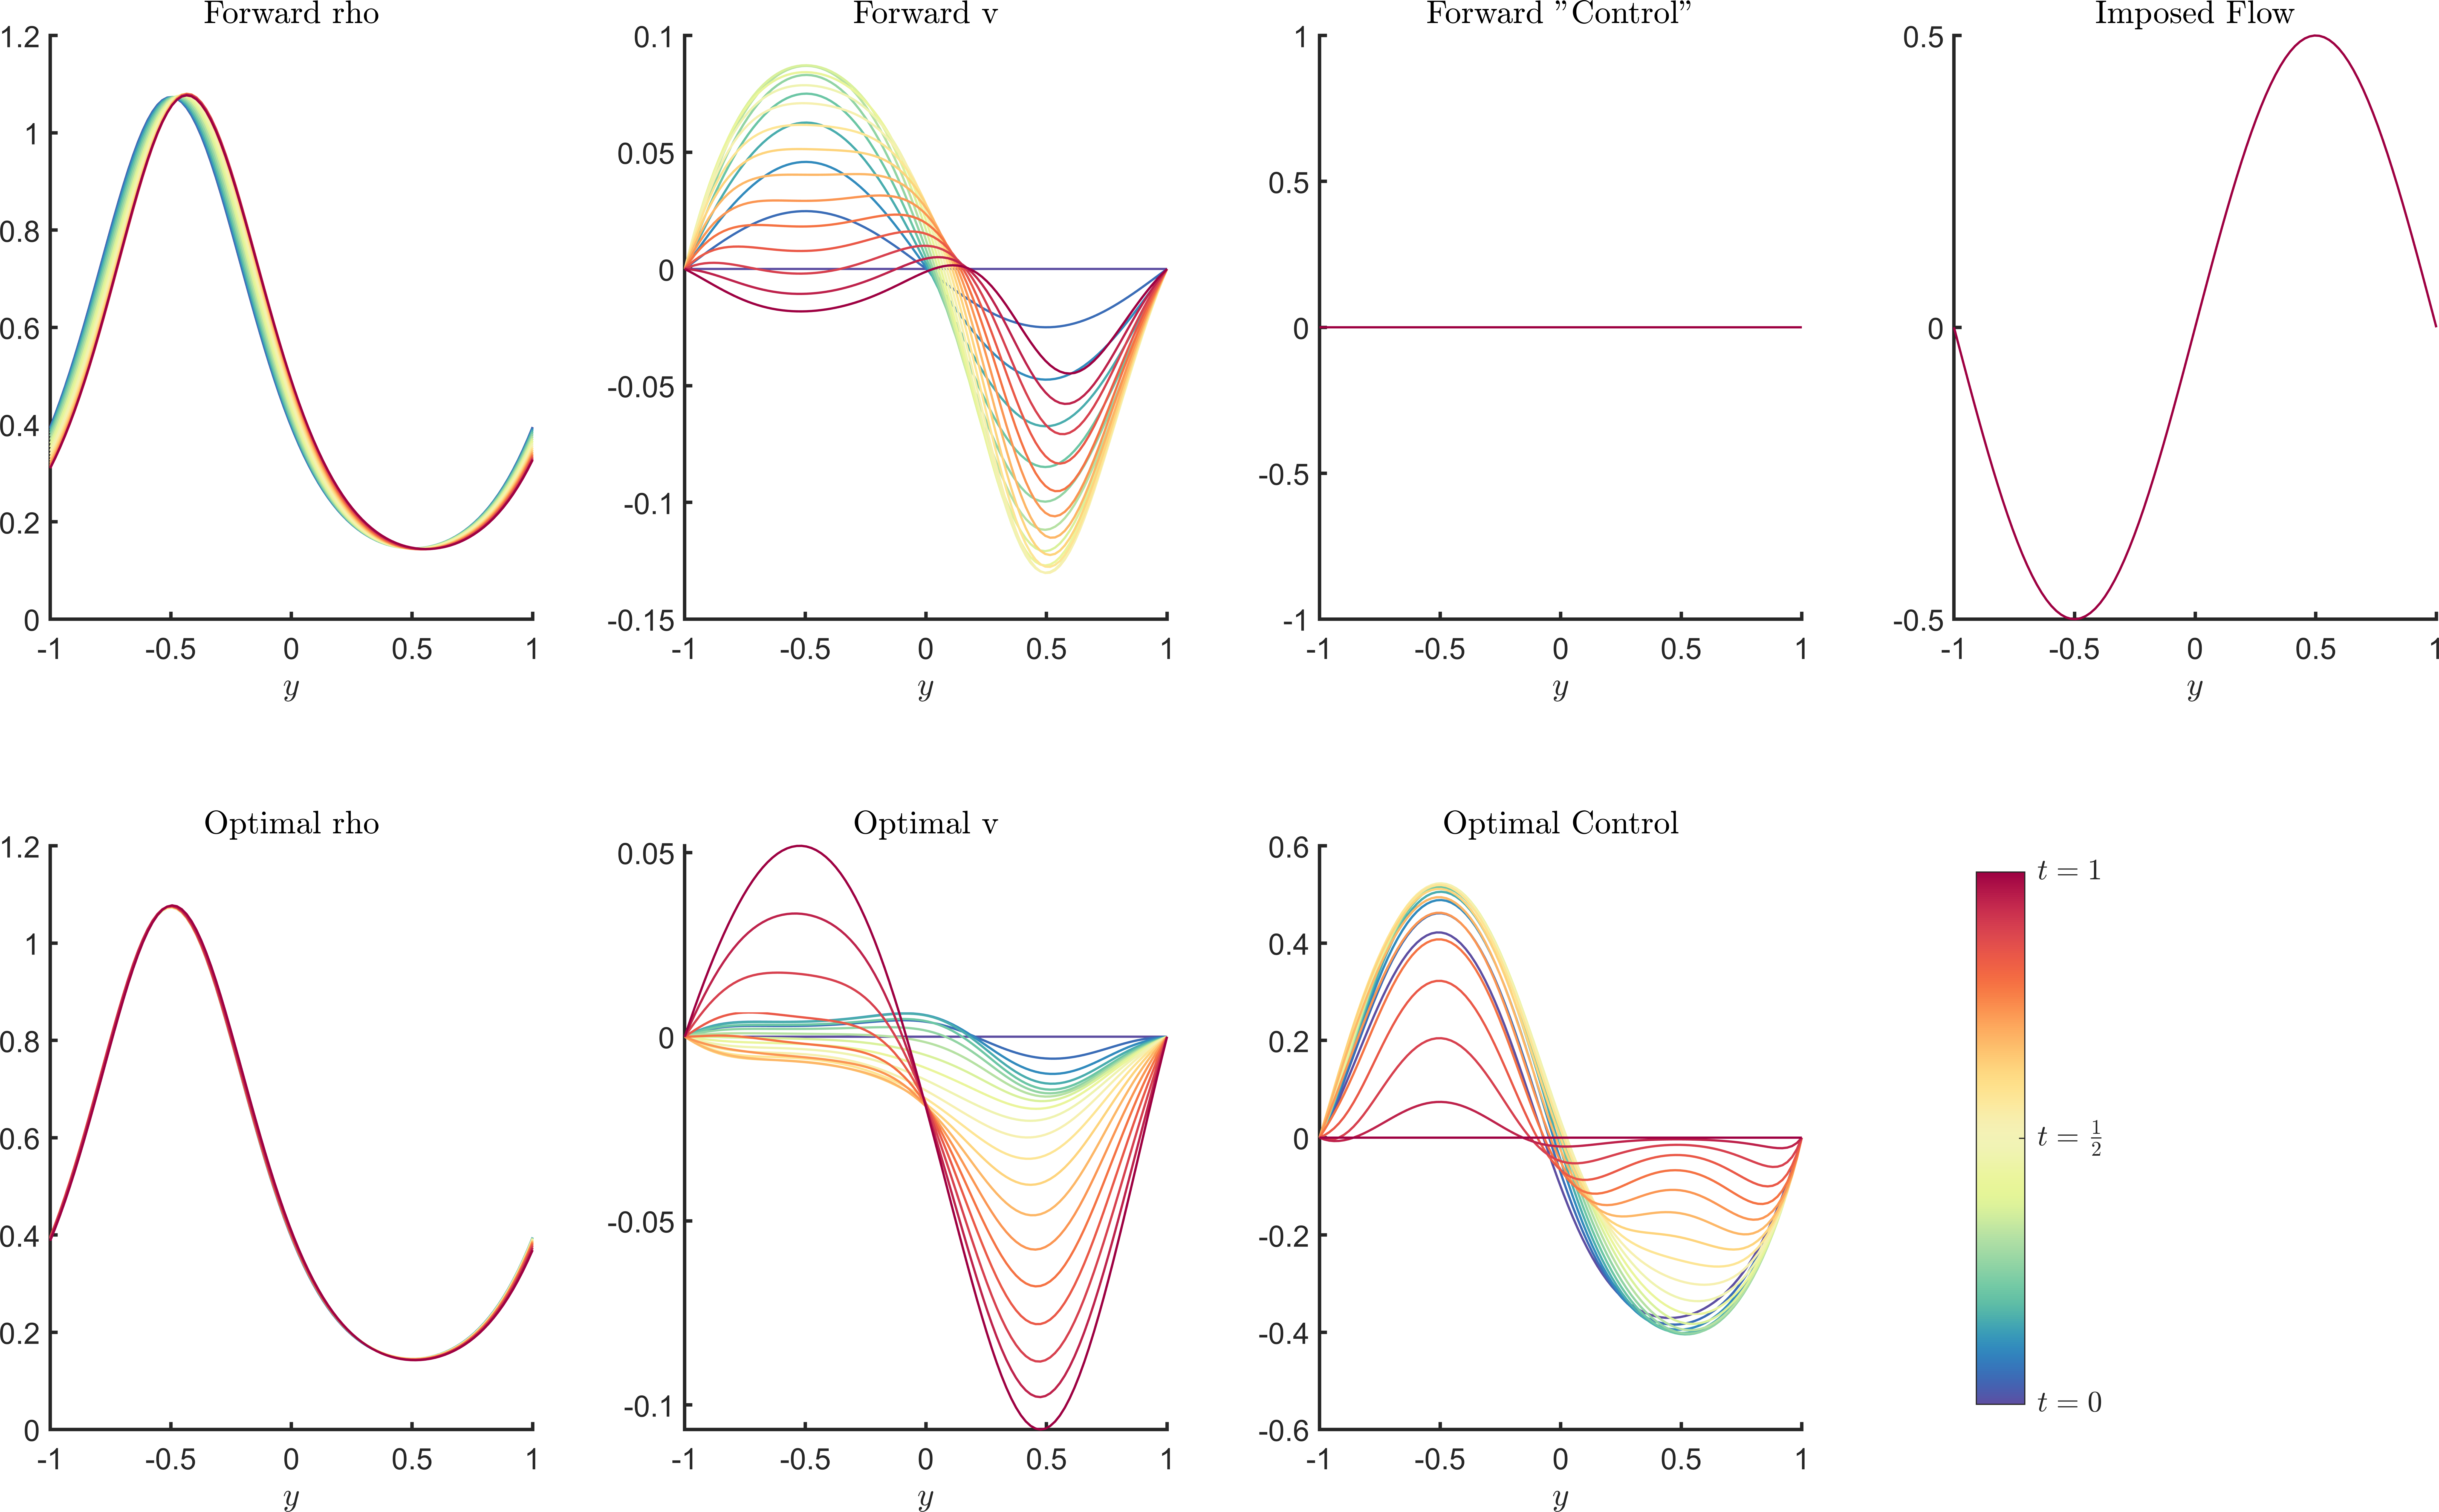
\includegraphics[scale=0.05]{Example1.png}
   	\caption{Example 1 ($\gamma = 1$, $\eta = 0.1$)}
   	\label{fig1}
   \end{figure}

    Next I tried to decrease both $\eta$ and $\gamma$ to see if I can break the numerics. With decreasing $\gamma$, the iterations are getting slower, but the number of iterations remains the same. We can set $\eta = 0$ without breaking the equations.
    The velocity profile, especially in the forward problem becomes steeper, as expected, but after a while, making $\gamma$ smaller (with $\eta = 0$) doesn't seem to make the chosen velocity profile steeper for this example.\\
    I can choose $\gamma = 0$ and $\eta =0$ in the problem and it converges. I am not sure whether that means that I chose a nice example or that something is wrong. We get $J_{FW}= 0.0052$ and $J_{Opt} = 9.2542\times 10^{-5}$. The result can be seen in Figure \ref{fig1a}.
    \begin{figure}
    	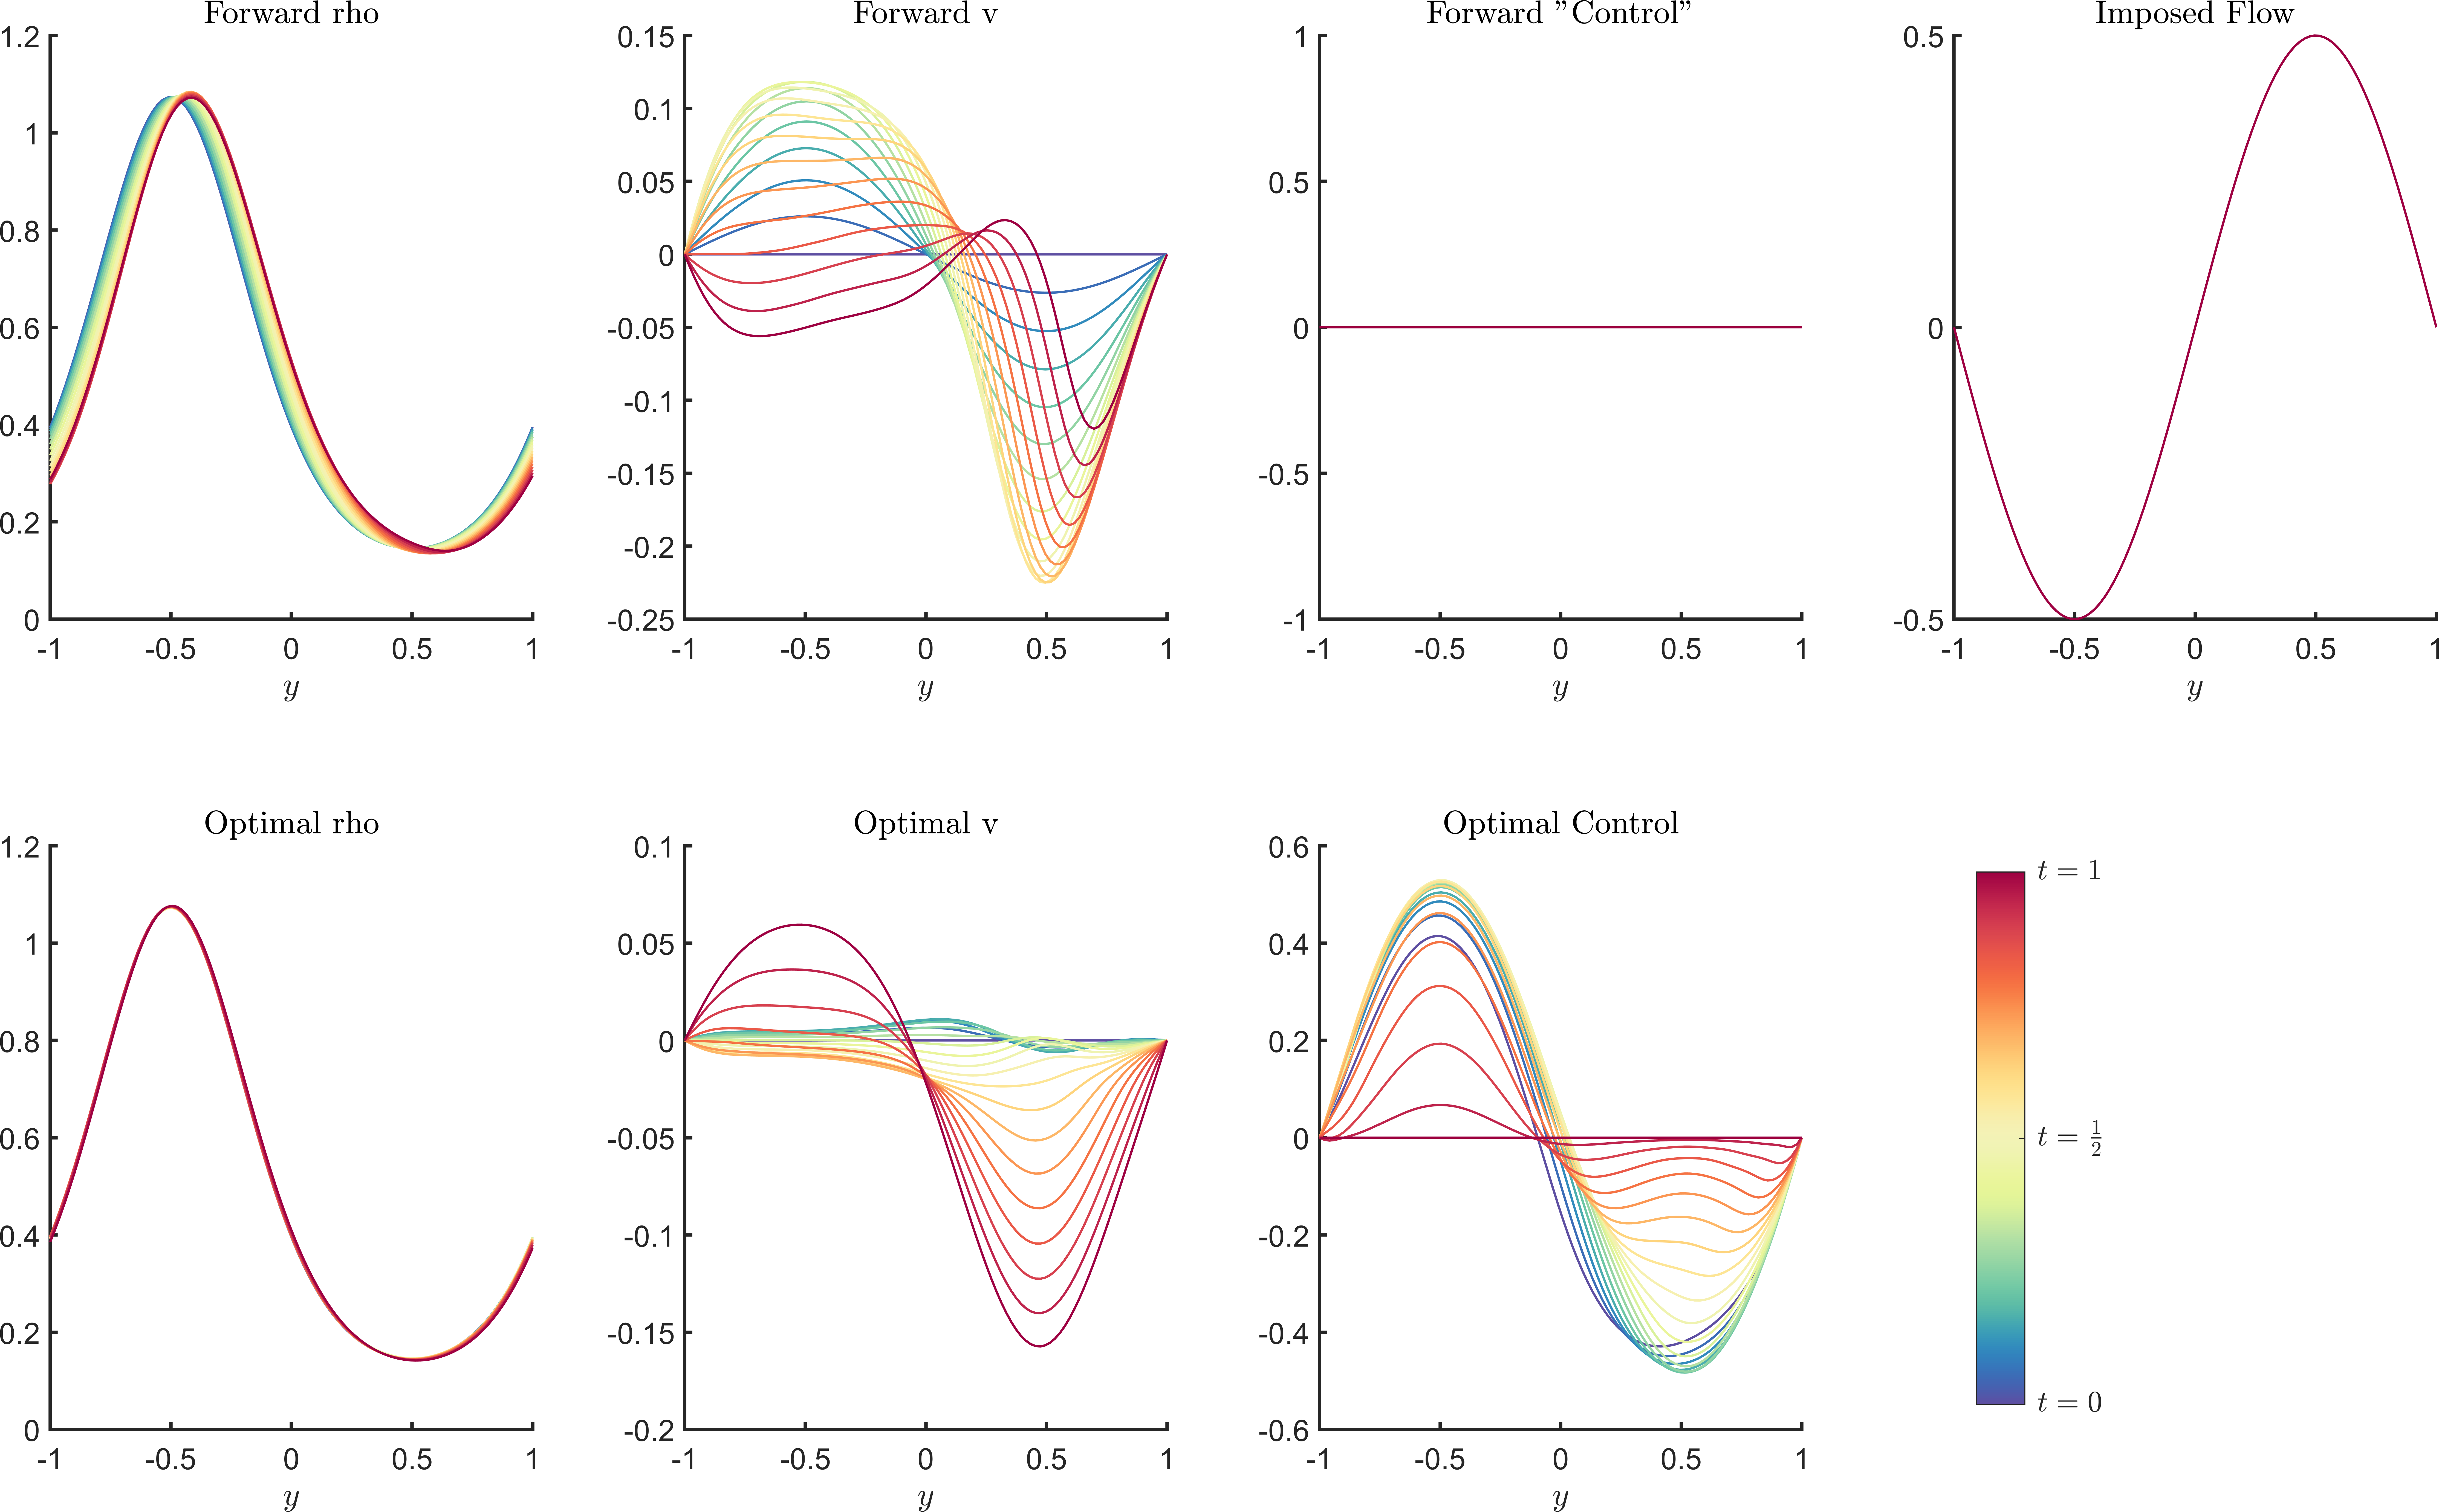
\includegraphics[scale=0.05]{Example1a.png}
    	\caption{Example 1a ($\gamma = 0$, $\eta = 0$)}
    	\label{fig1a}
    \end{figure}
    
    Choosing the middle ground with $\eta = 0.01$ and $\gamma =0.1$,we get $J_{FW} = 0.0049$ and $J_{Opt} = 9.2244 \times 10^{-5}$, see Figure \ref{fig1b}. Increasing the number of points to $n = 30$, $N = 50$ does not change the results. Running this example with $\beta = 10^{-1}$ gives $J_{Opt} = 0.0027$. The optimal velocity and control look different from the lower $\beta$ case, as expected, see Figure \ref{fig1b1}.
	\begin{figure}
		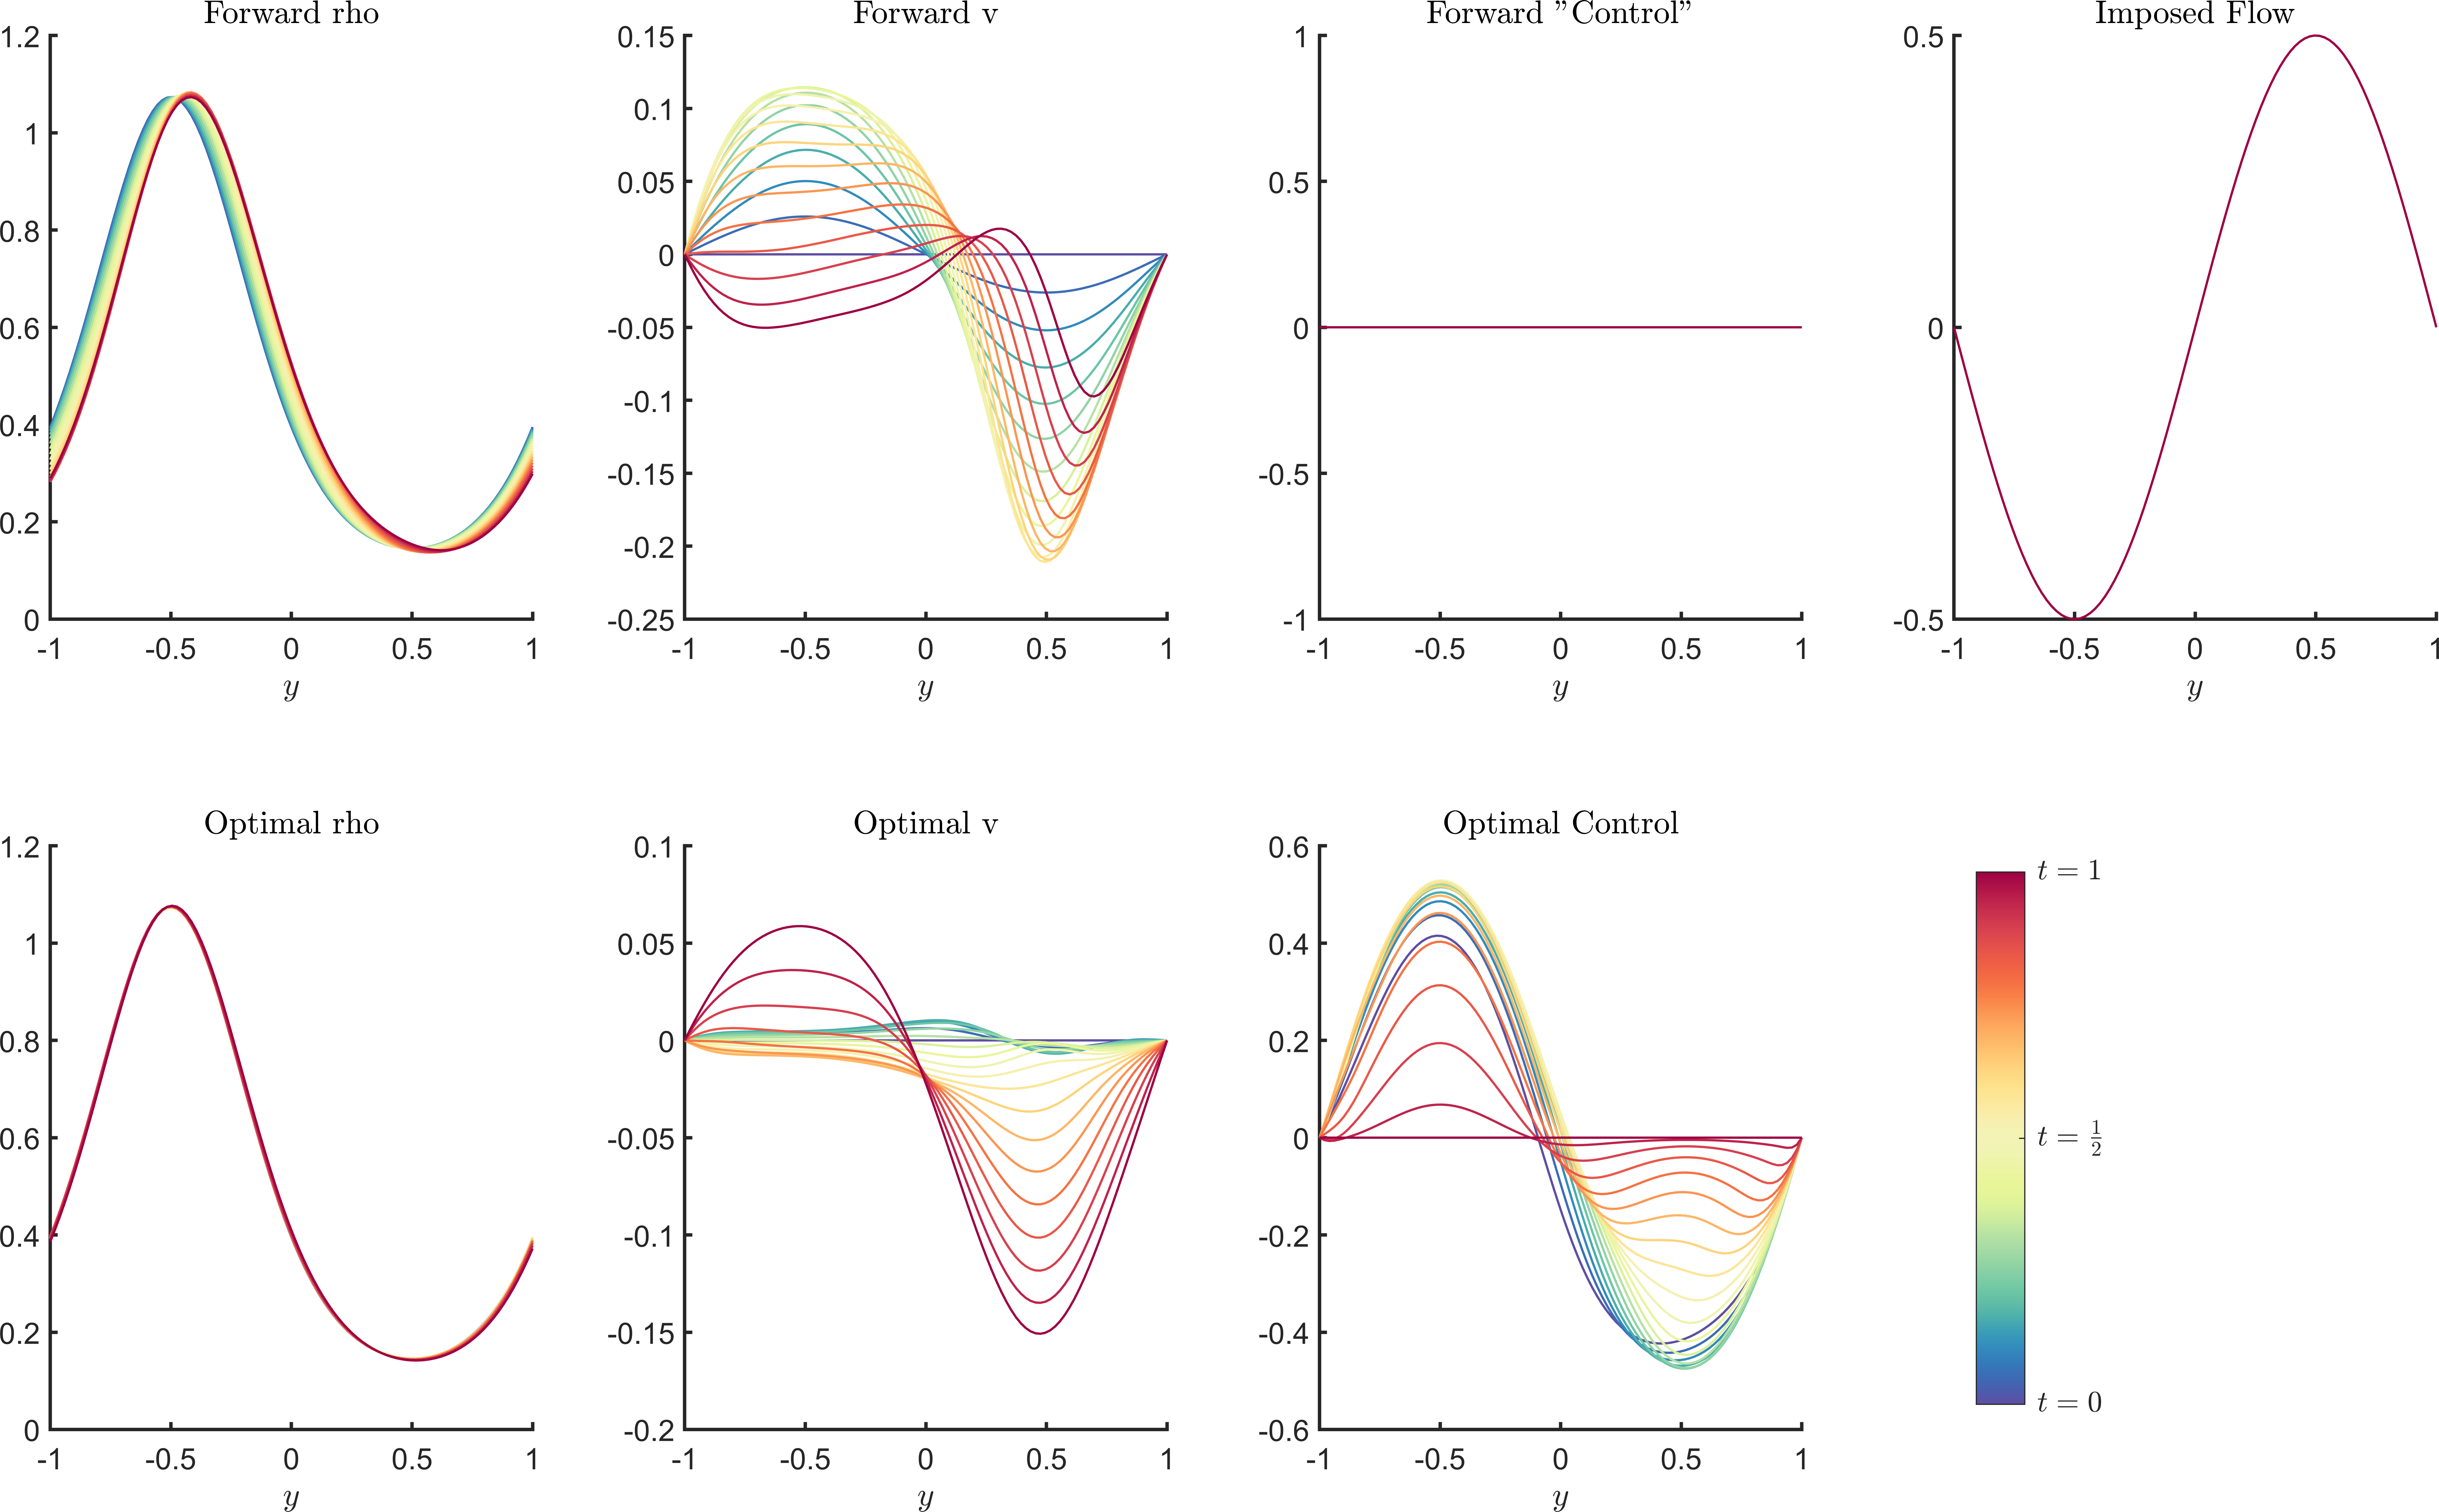
\includegraphics[scale=0.05]{Example1b.png}
		\caption{Example 1b ($\gamma = 0.1$, $\eta = 0.01$)}
		\label{fig1b}
	\end{figure}   
\begin{figure}
	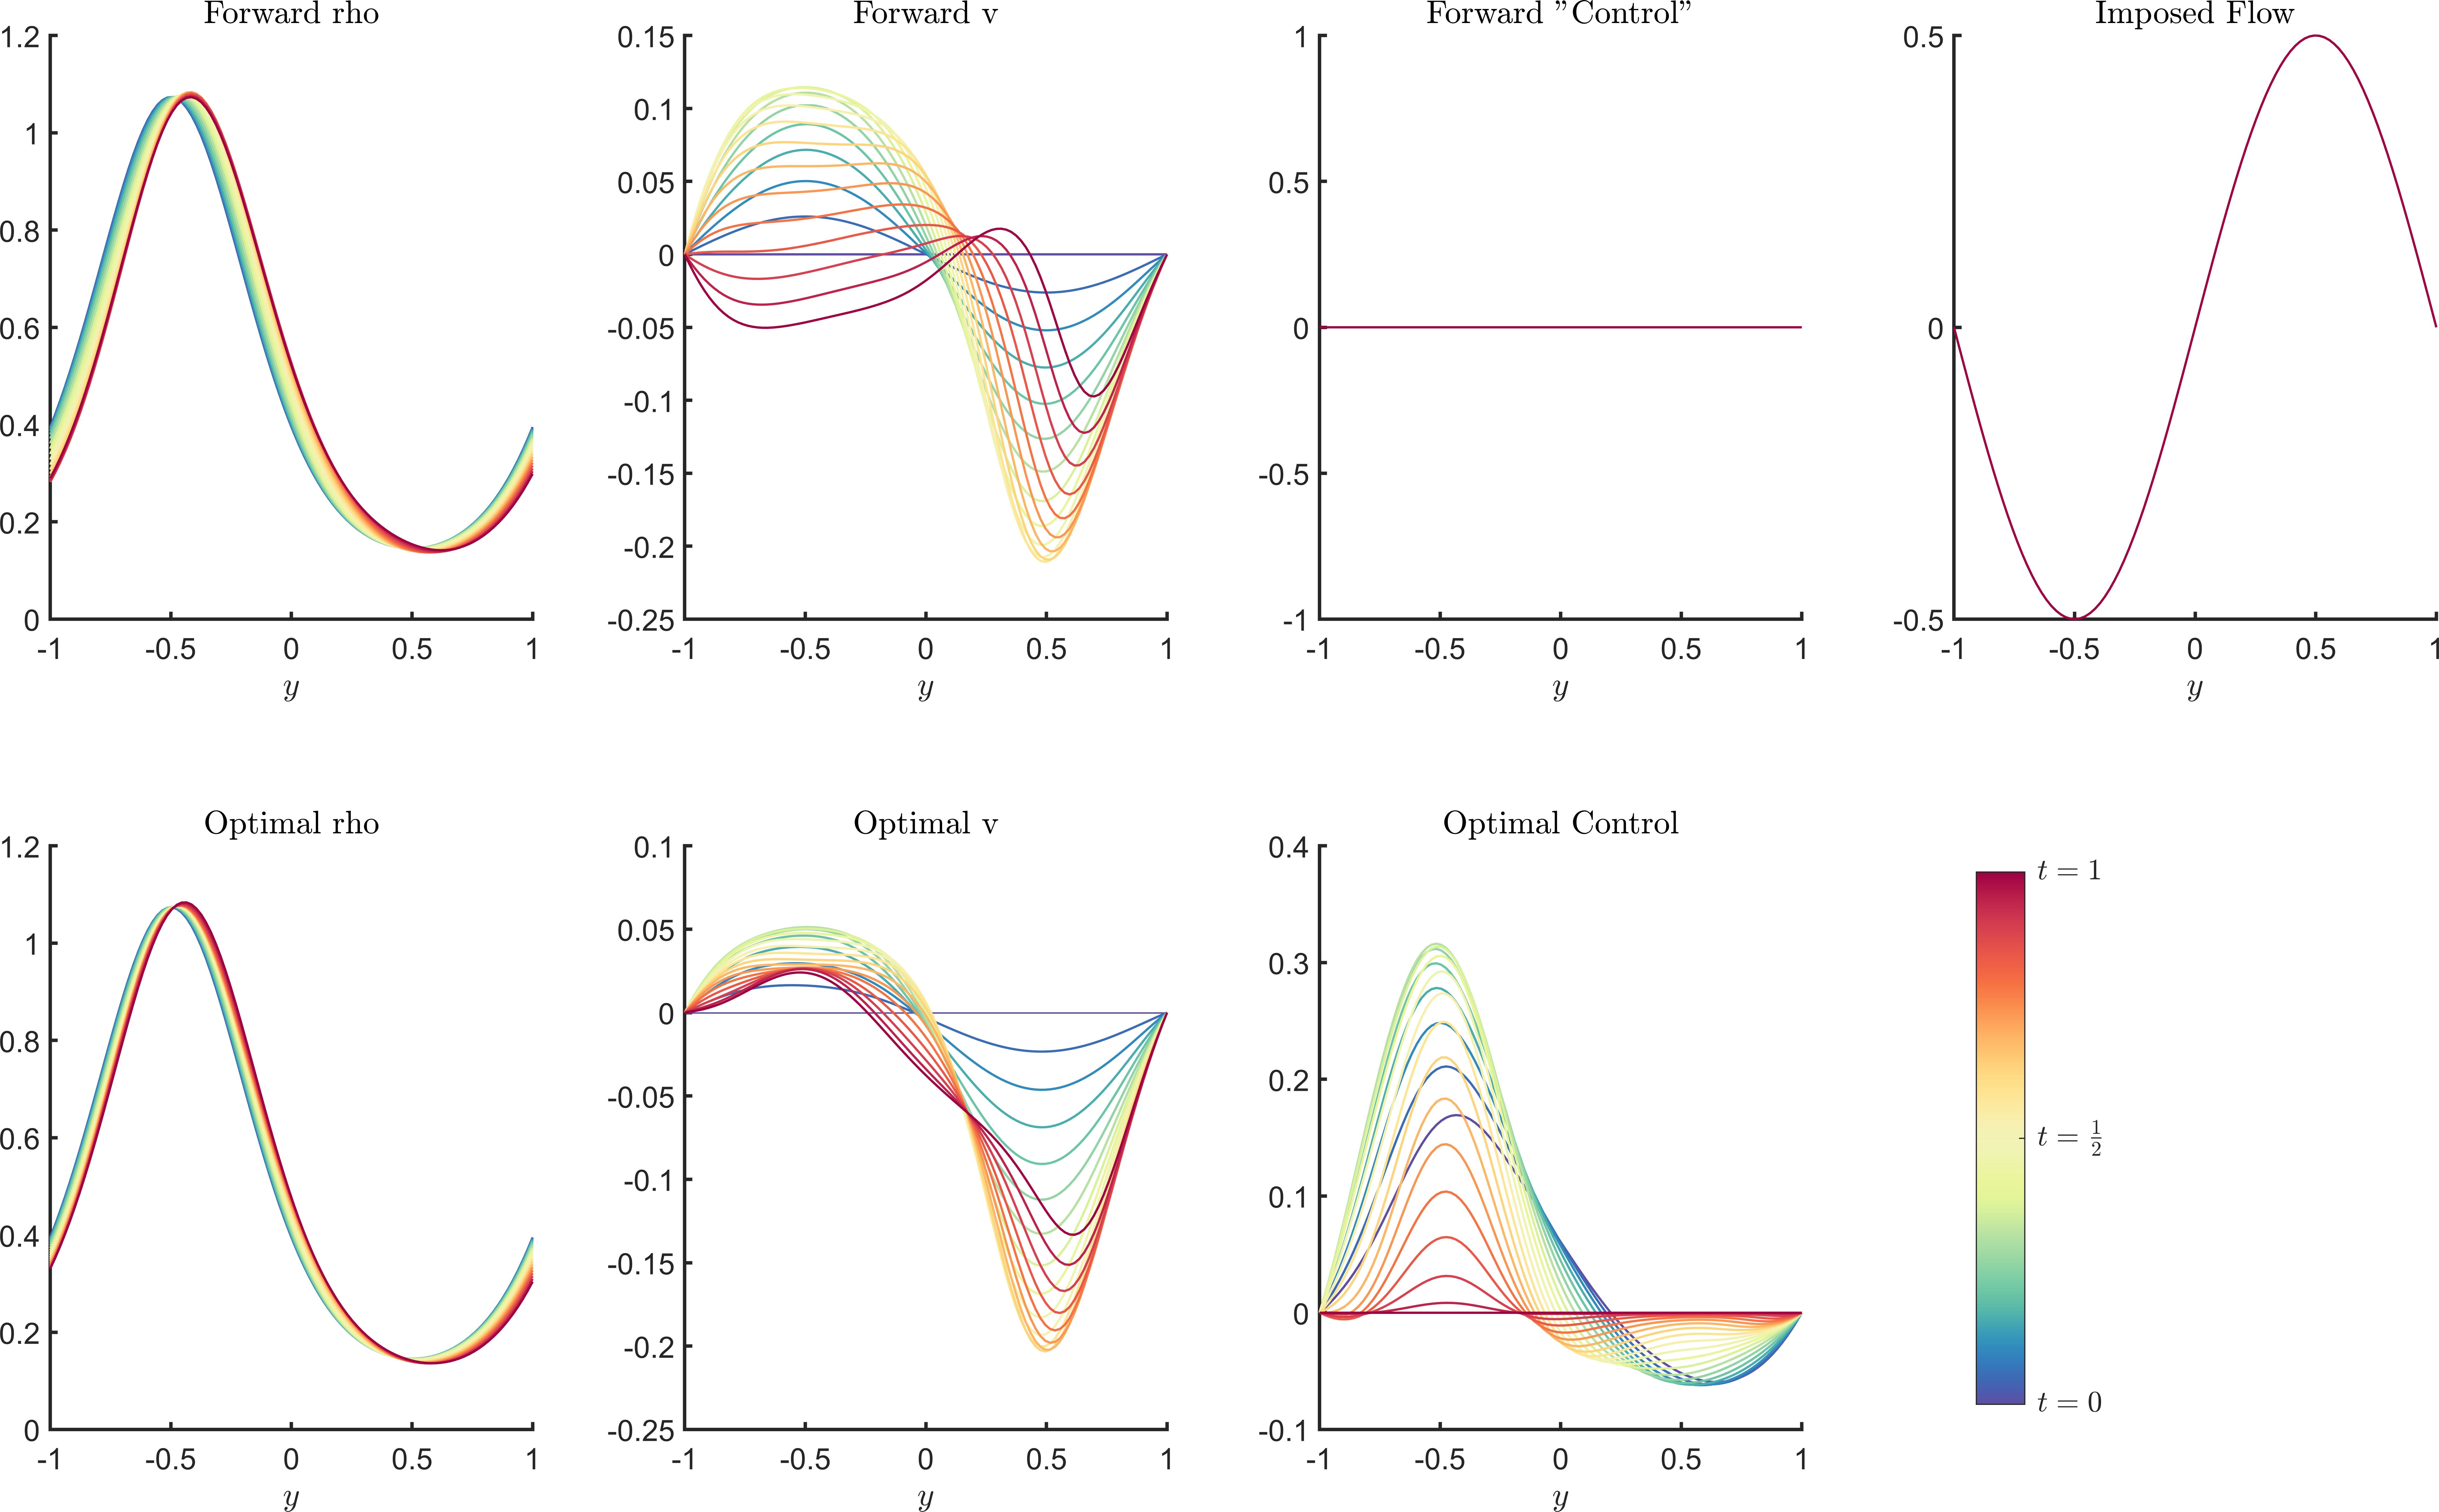
\includegraphics[scale=0.05]{Example1b1.png}
	\caption{Example 1b.1 ($\gamma = 0.1$, $\eta = 0.01$, $\beta = 10^{-1}$)}
	\label{fig1b1}
\end{figure}
	   
    Increasing $\eta$ to $0.5$ makes the velocity gradients less steep, as expected. We get $J_{FW} = 0.0017$, $J_{Opt} = 7.9641 \times 10^{-5}$, see Figure \ref{fig1c}. 
    \begin{figure}
    	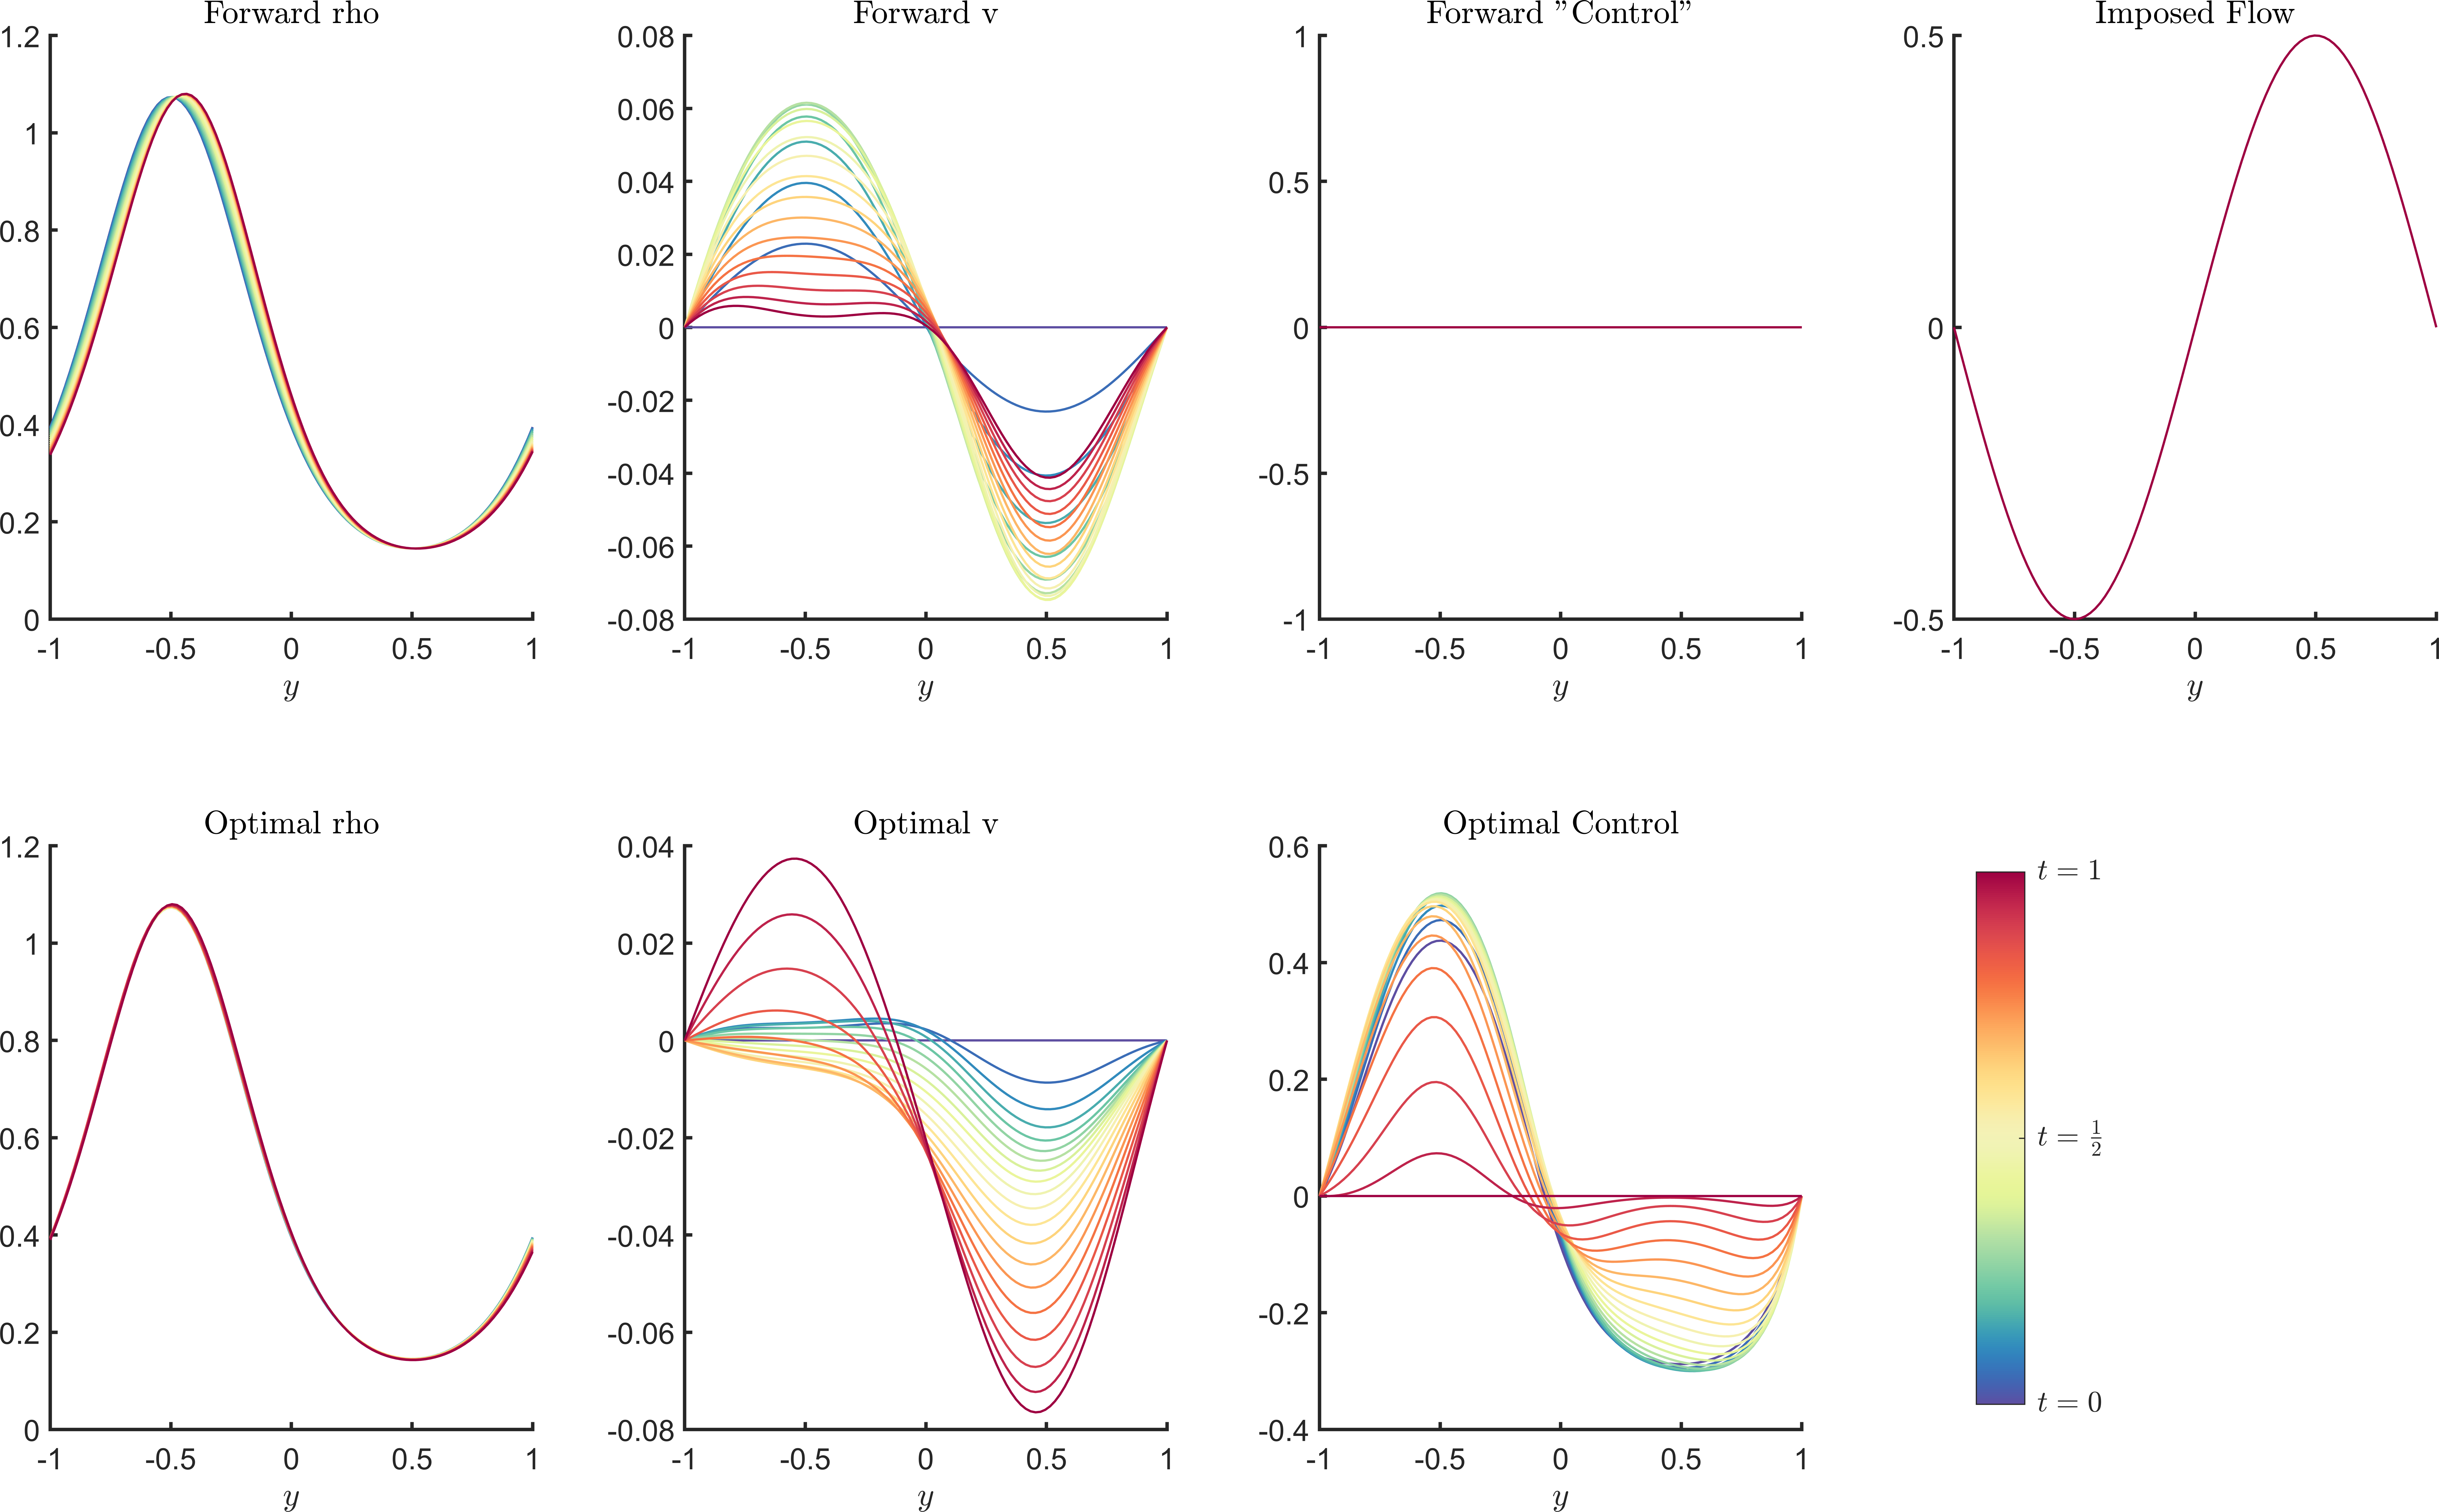
\includegraphics[scale=0.05]{Example1c.png}
    	\caption{Example 1c ($\gamma = 0.1$, $\eta = 0.5$)}
    	\label{fig1c}
    \end{figure} 	   


In all the above examples it can be seen that the optimal control is doing exactly as expected. It acts in the opposite direction to the imposed flow and with similar magnitude and shape. The difference is that the optimal control has to go to zero at the final time, while the imposed flow $\Con$ stays constant. This is reflected in the optimal $v$ as well. During most of the time horizon it stays close to zero, the steady state, while in the later times, it varies from zero.

\subsection{Second Test Problem}
We choose a different imposed flow to above, but asking for the same steady state as target:
   \begin{align*}
&\Sta_0 = \hat \Sta =  \frac{1}{2.5321}e^{-\sin(\pi y)}, \ \ V^{ext} = \sin(\pi y)\\
&\Stav = \mathbf{0}, \ \  \mathbf{w} = \mathbf{0}\\
&\Con = 1/2\cos(\pi y) + 1/2
\end{align*}
	
First we choose $\gamma = 0.1$, $\eta = 0.01$ and $\beta = 10^{-3}$ with again $n = 20$, $N=30$. $J_{FW} = 0.0096$, $J_{Opt} = 2.6320 \times 10^{-4}$, see Figure \ref{fig2}. It can be seen that the optimal control is again acting opposite to the imposed flow, which is different from the one in Example 1. We can also see that the forward velocity is already really steep at late times. It turns out that for $\gamma = 0.01$, $\eta = 0.01$, we need more points to get a numerically stable forward problem. With $n = 30$ and $N = 50$, we get $J_{FW} = 0.0101$, $J_{Opt} = 2.6365 \times 10^{-4}$, see Figure \ref{fig2a}. While it needs more points, the result is not qualitatively different from the case with larger $\gamma$.

    \begin{figure}
		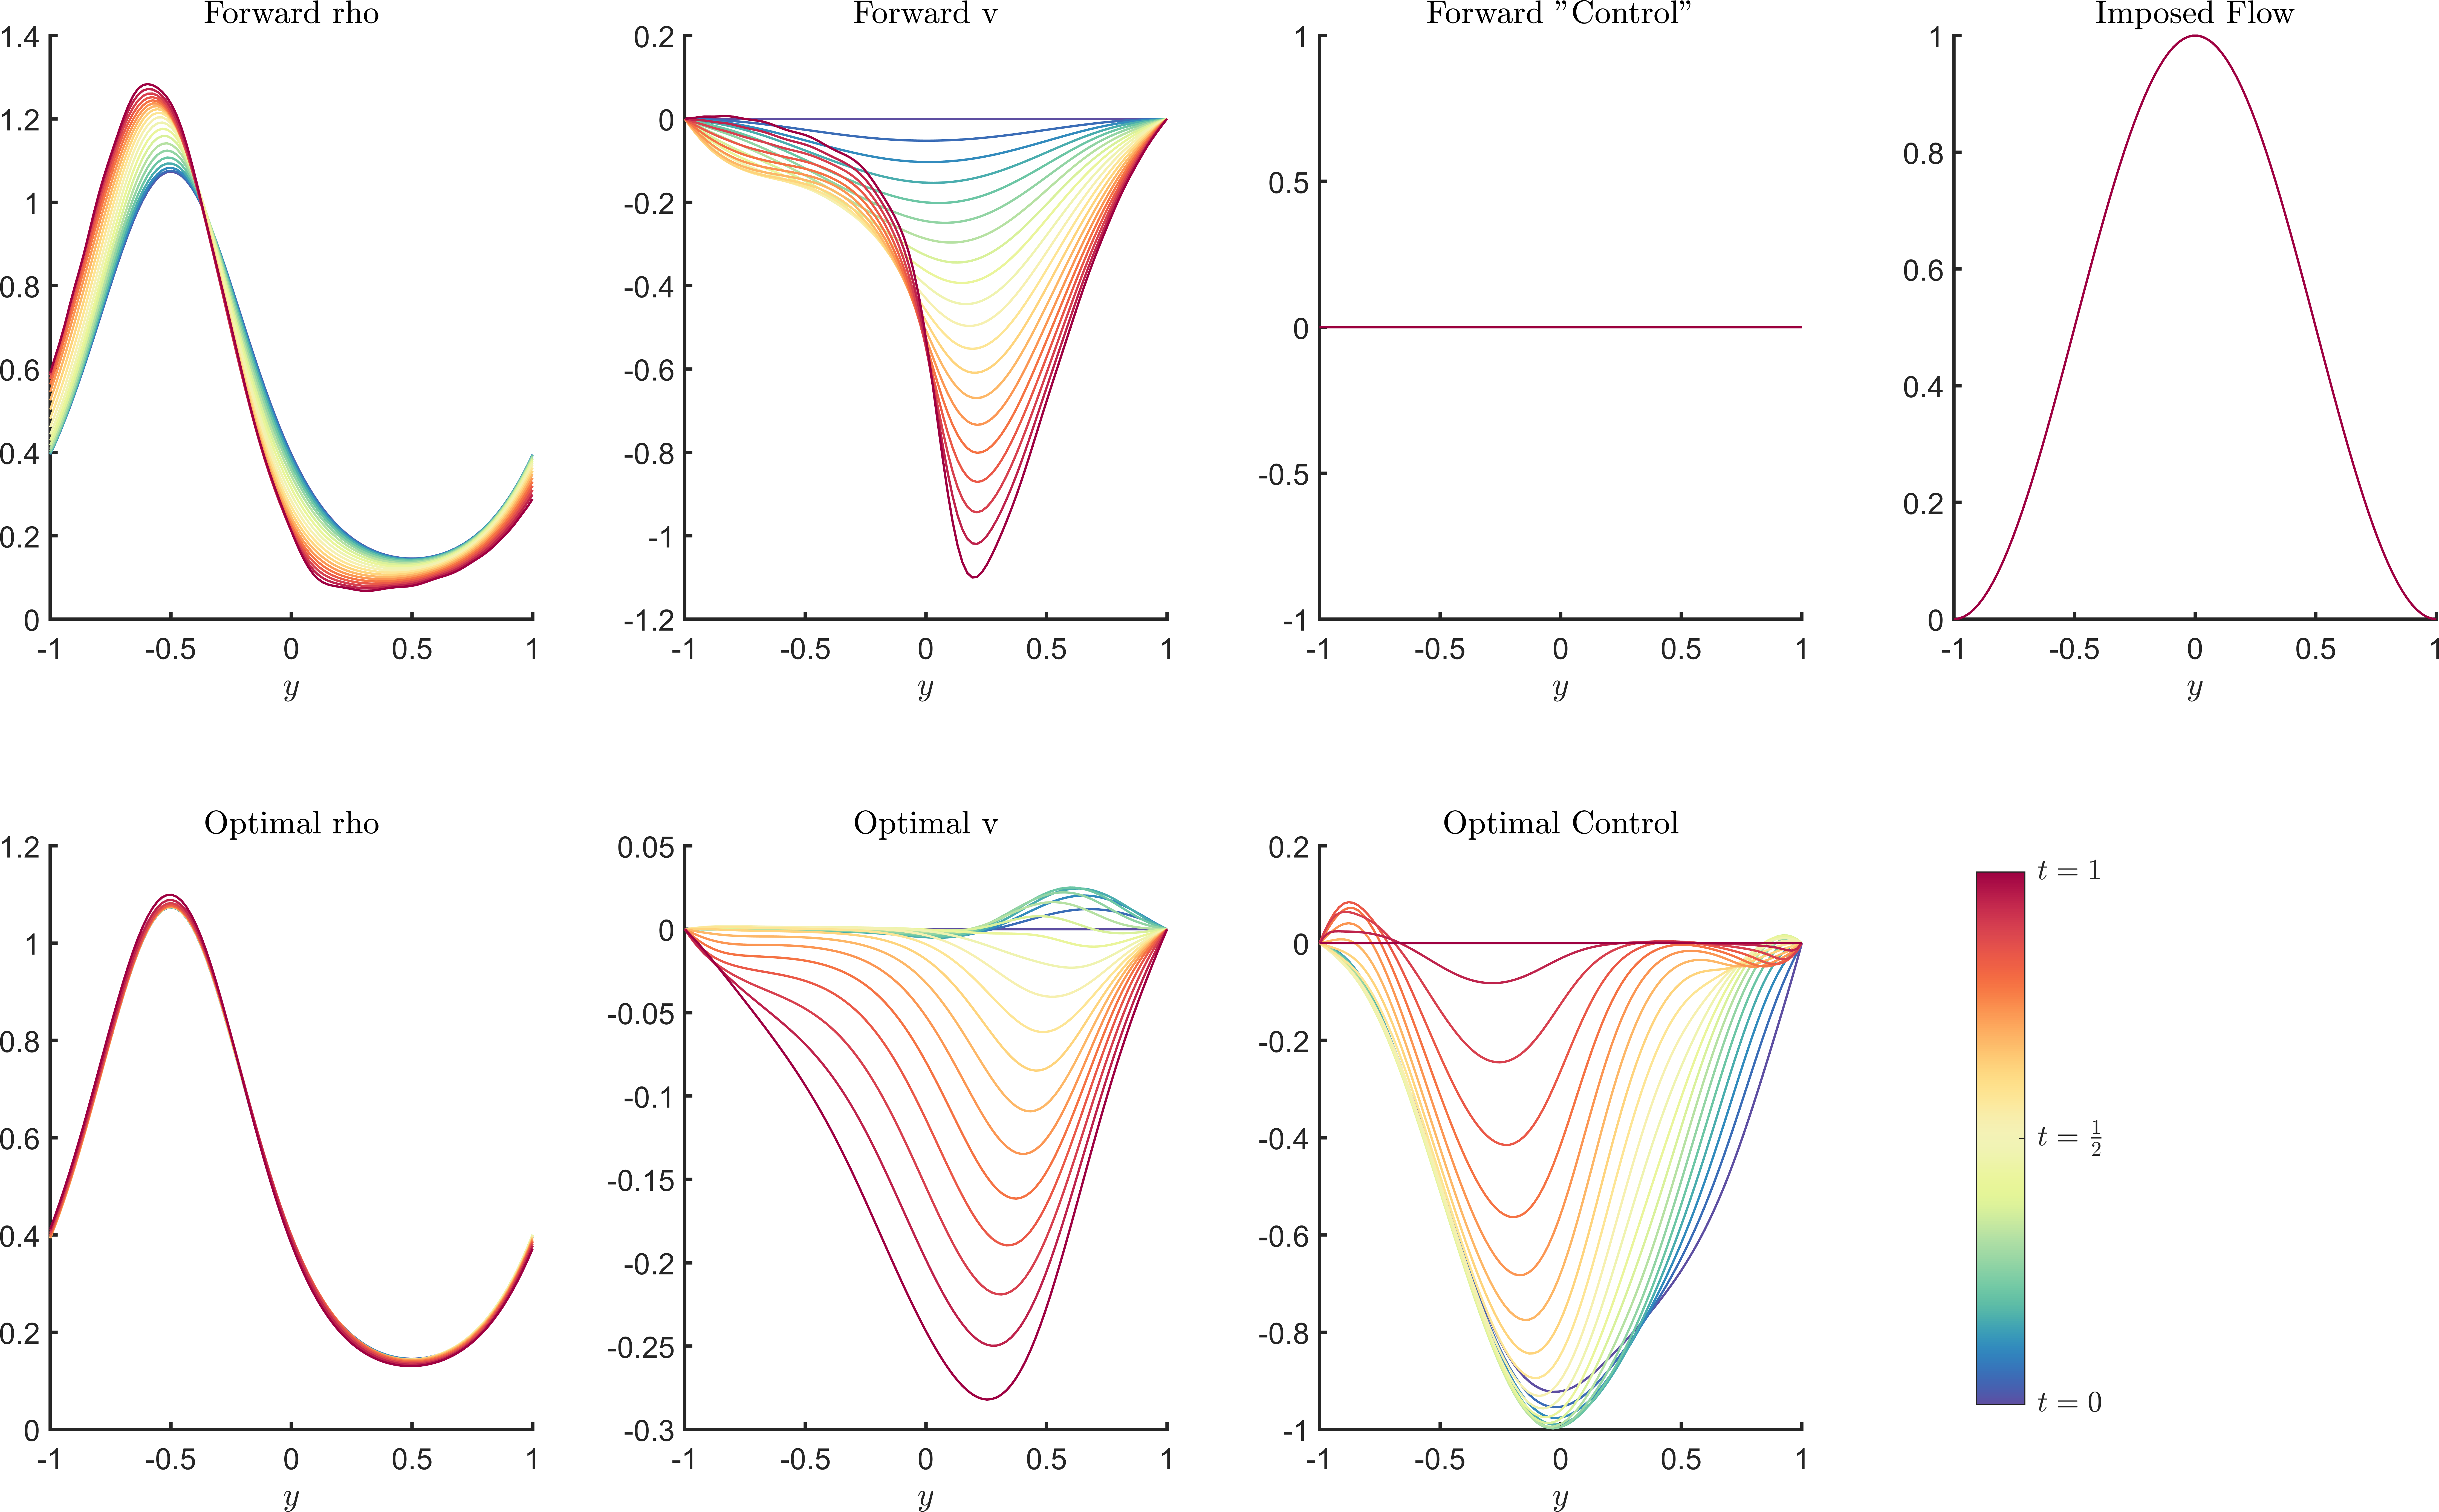
\includegraphics[scale=0.05]{Example2.png}
		\caption{Example 2 ($\gamma = 0.1$, $\eta = 0.01$)}
		\label{fig2}
    \end{figure} 
    \begin{figure}
		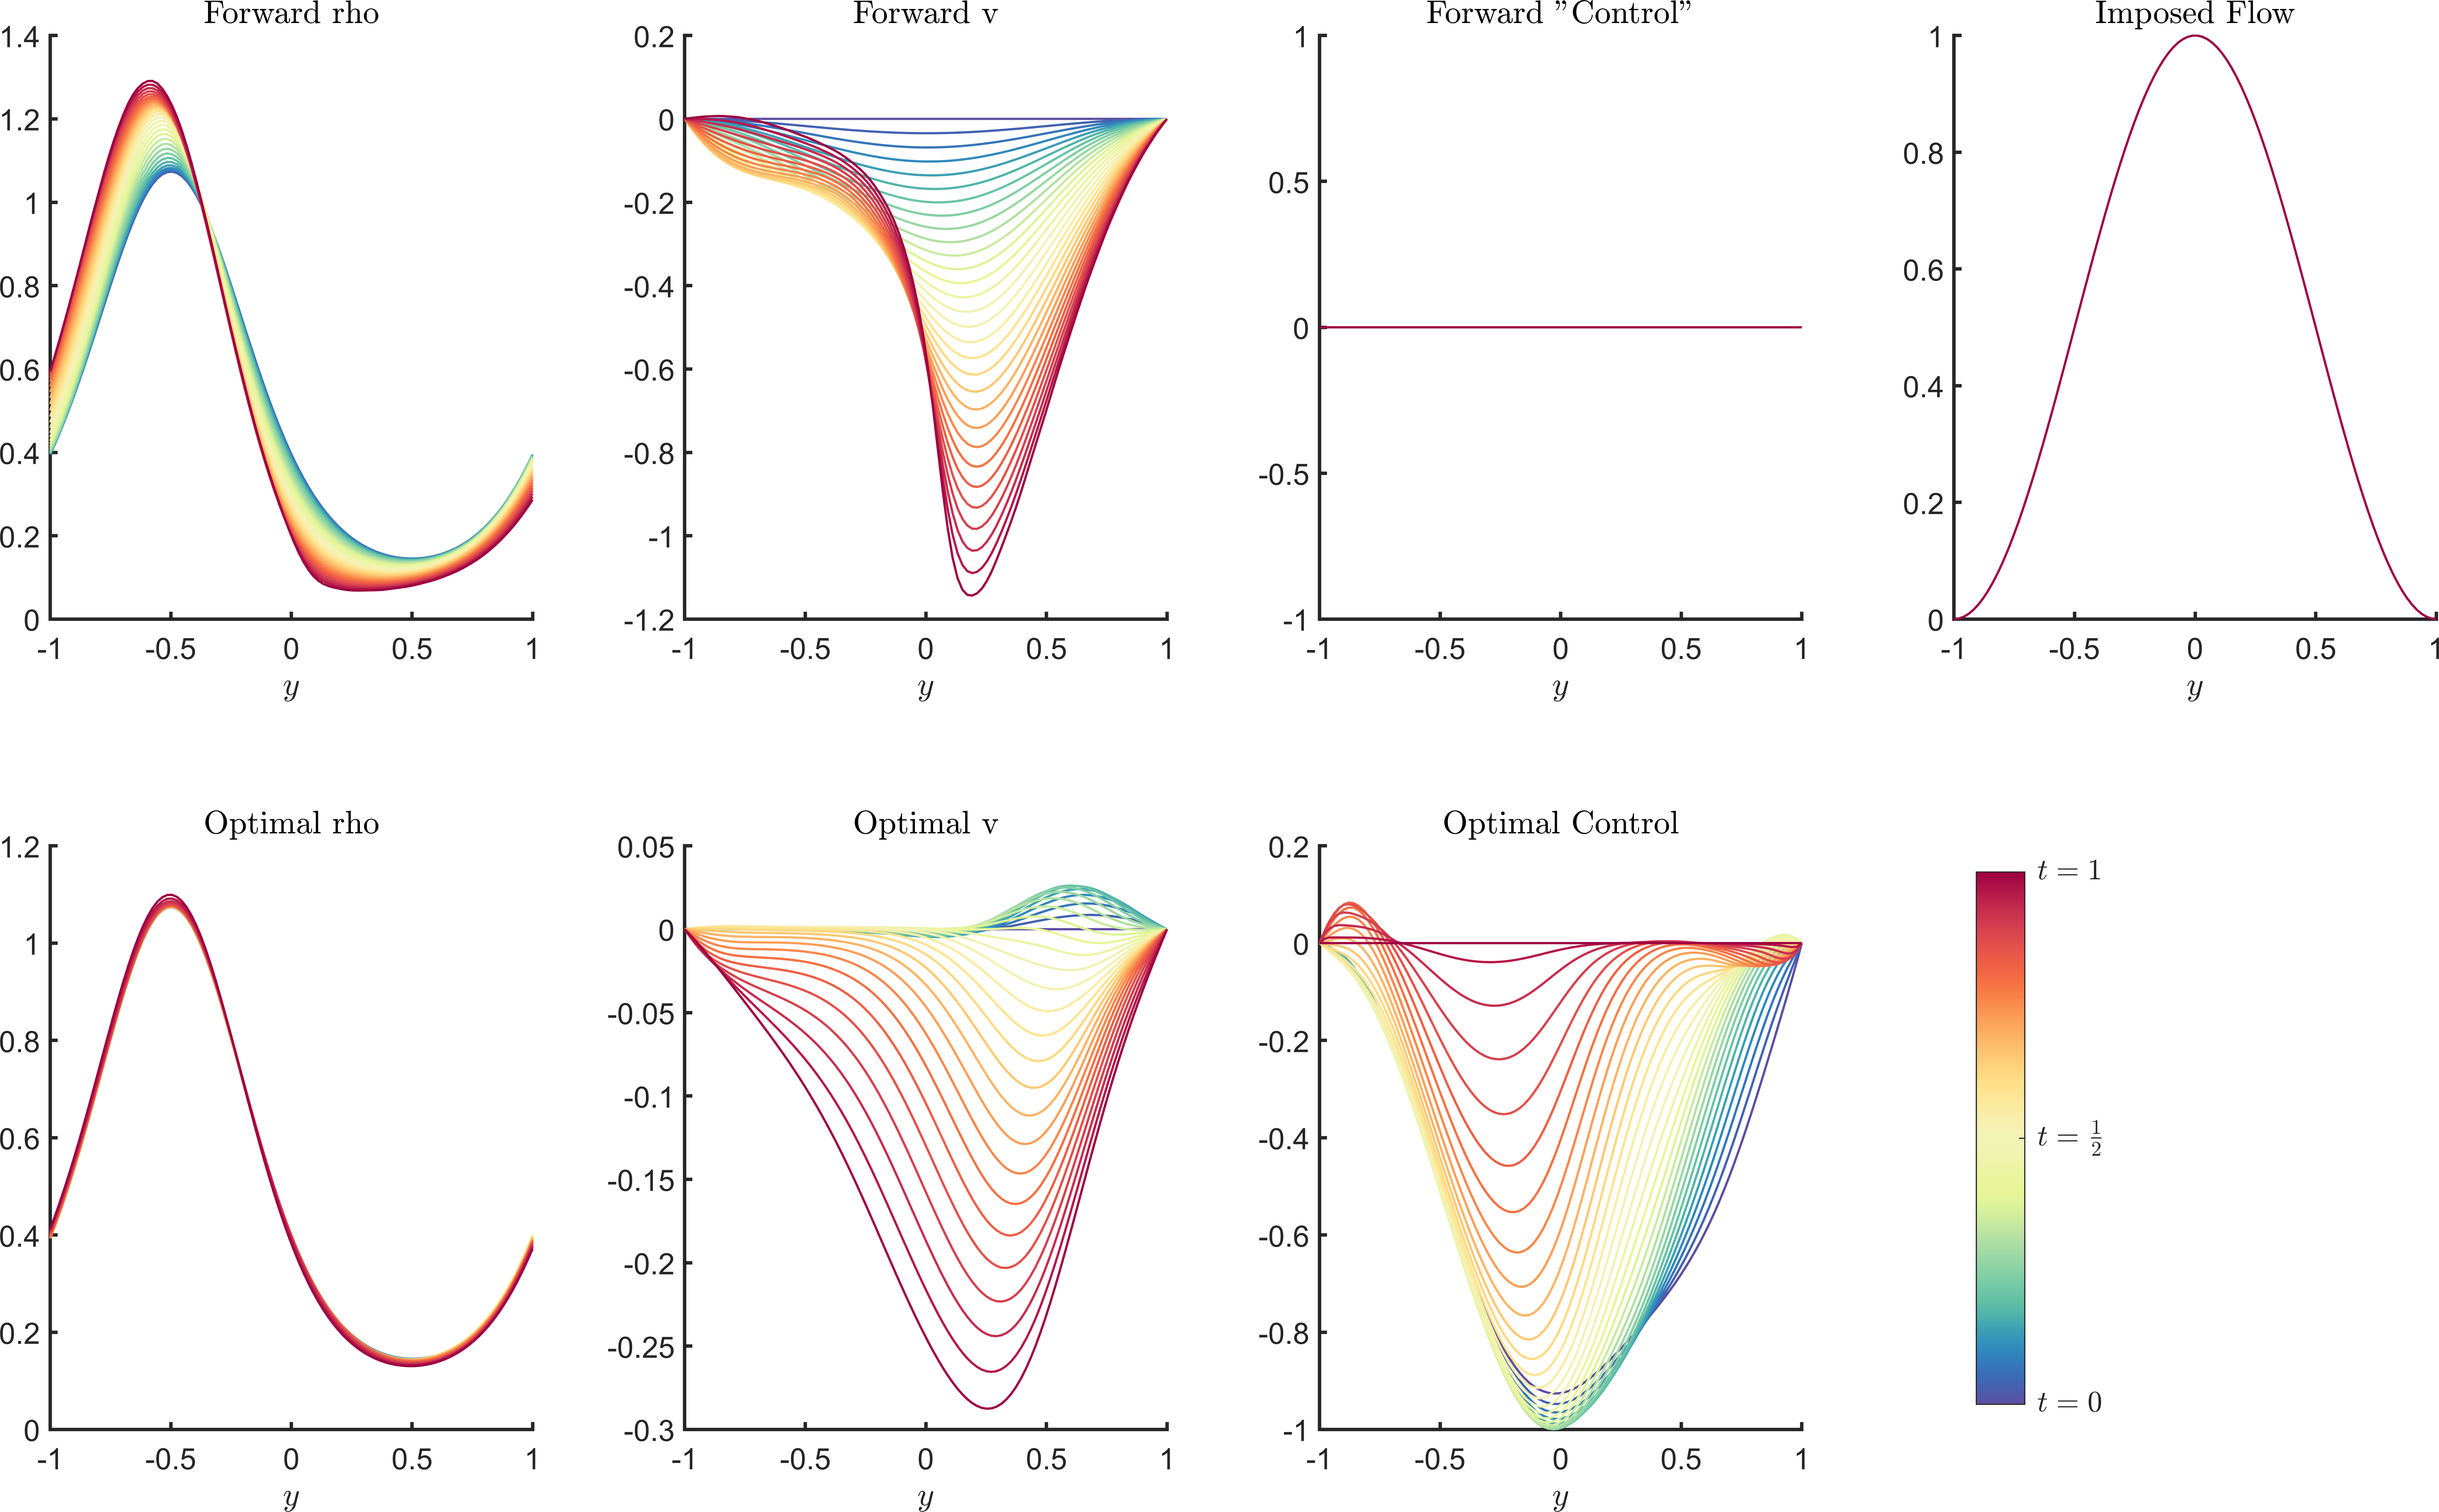
\includegraphics[scale=0.05]{Example2a.png}
		\caption{Example 2a ($\gamma = 0.01$, $\eta = 0.01$)}
		\label{fig2a}
    \end{figure} 

\subsection{Third Test Problem}
We now go back to the imposed flow from Problem 1 and change the target for $\Sta$.
We choose:
\begin{align*}
&\Sta_0 = \hat \Sta = \frac{1}{2.0507}e^{-0.5 \frac{2}{3 \pi}\sin((3/2)\pi y)}, \ \ V^{ext} =0.5 \frac{2}{3 \pi}\sin((3/2)\pi y)\\
&\Stav = \mathbf{0}, \ \  \mathbf{w} = \mathbf{0}\\
&\Con = 0.5 \sin(\pi y) 
\end{align*}
At first choose $\gamma = 0.1$, $\eta = 0.1$, $\beta = 10^{-3}$. Then $J_{FW} = 0.0031$, $J_{Opt} = 9.9376\times 10^{-5}$ and Figure \ref{fig3} shows the result. 
    \begin{figure}
		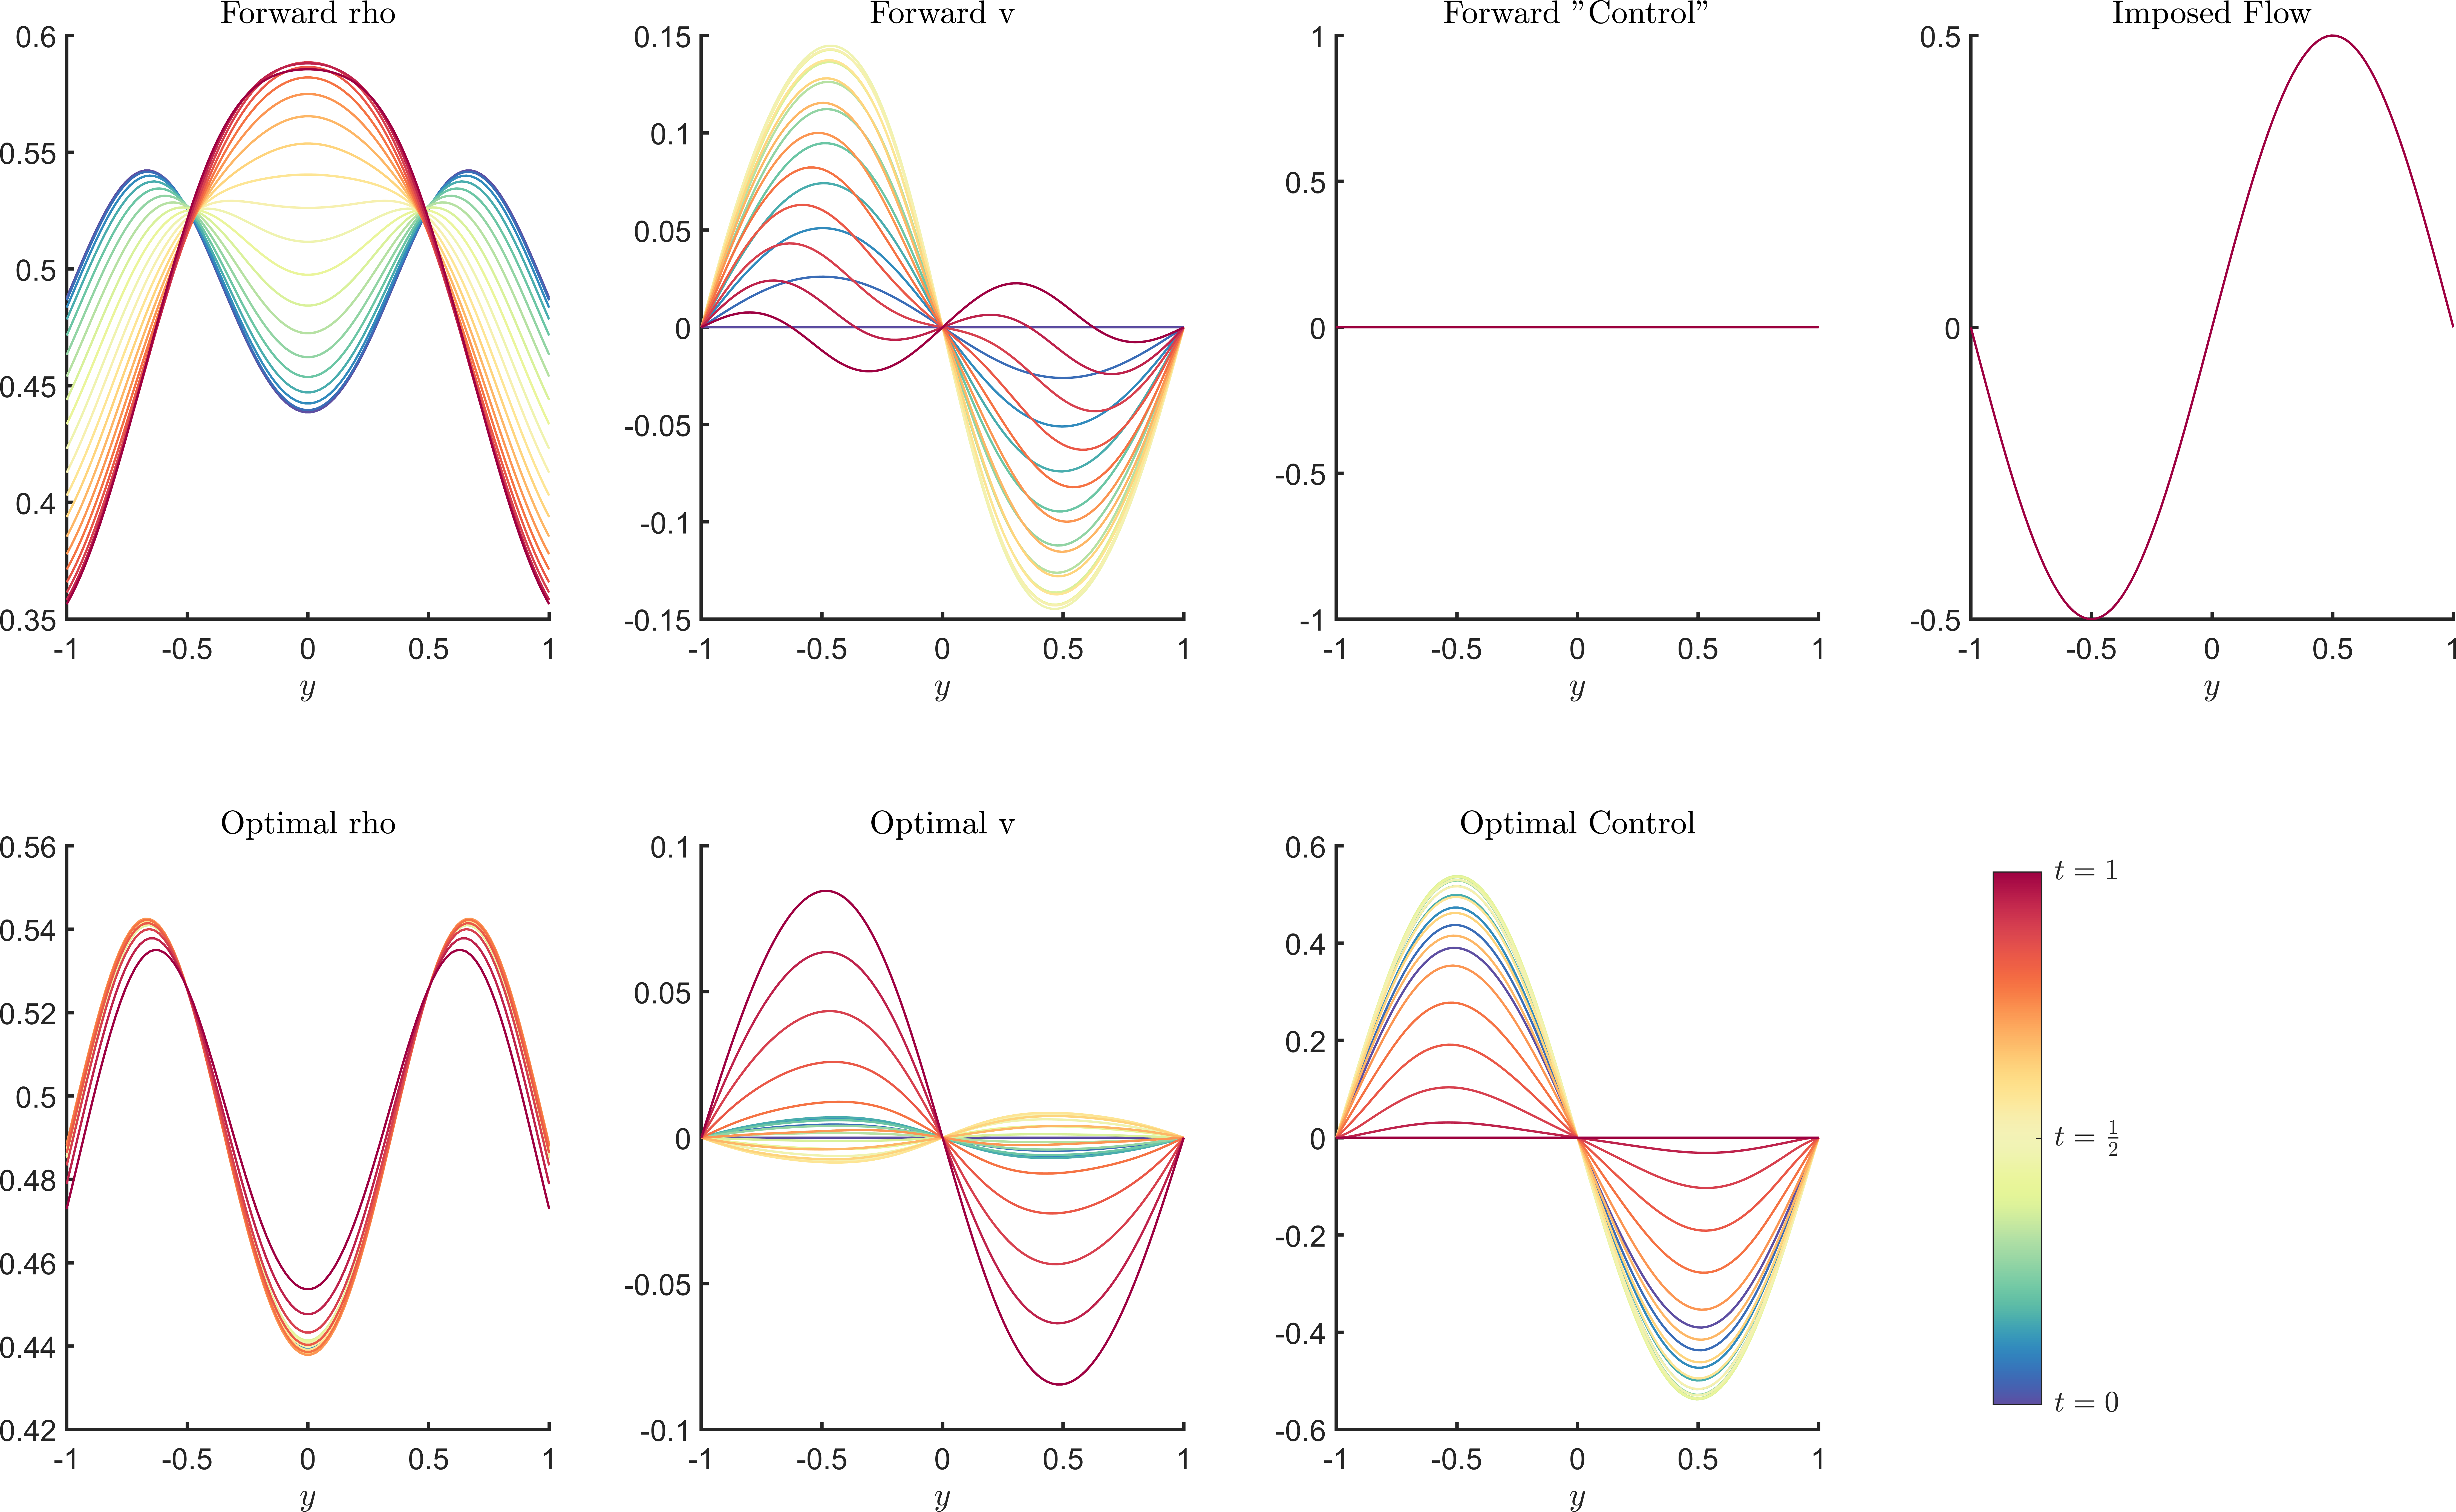
\includegraphics[scale=0.05]{Example3.png}
		\caption{Example 3 ($\gamma = 0.1$, $\eta = 0.1$)}
		\label{fig3}
    \end{figure} 
Then set $\gamma = 0.1$, $\eta = 0.01$, $\beta = 10^{-3}$. Then $J_{FW} = 0.0043$, $J_{Opt} = 9.9954\times 10^{-5}$ and Figure \ref{fig3a} shows the result. I think this looks the same as for the above case with larger $\eta$.
\begin{figure}
	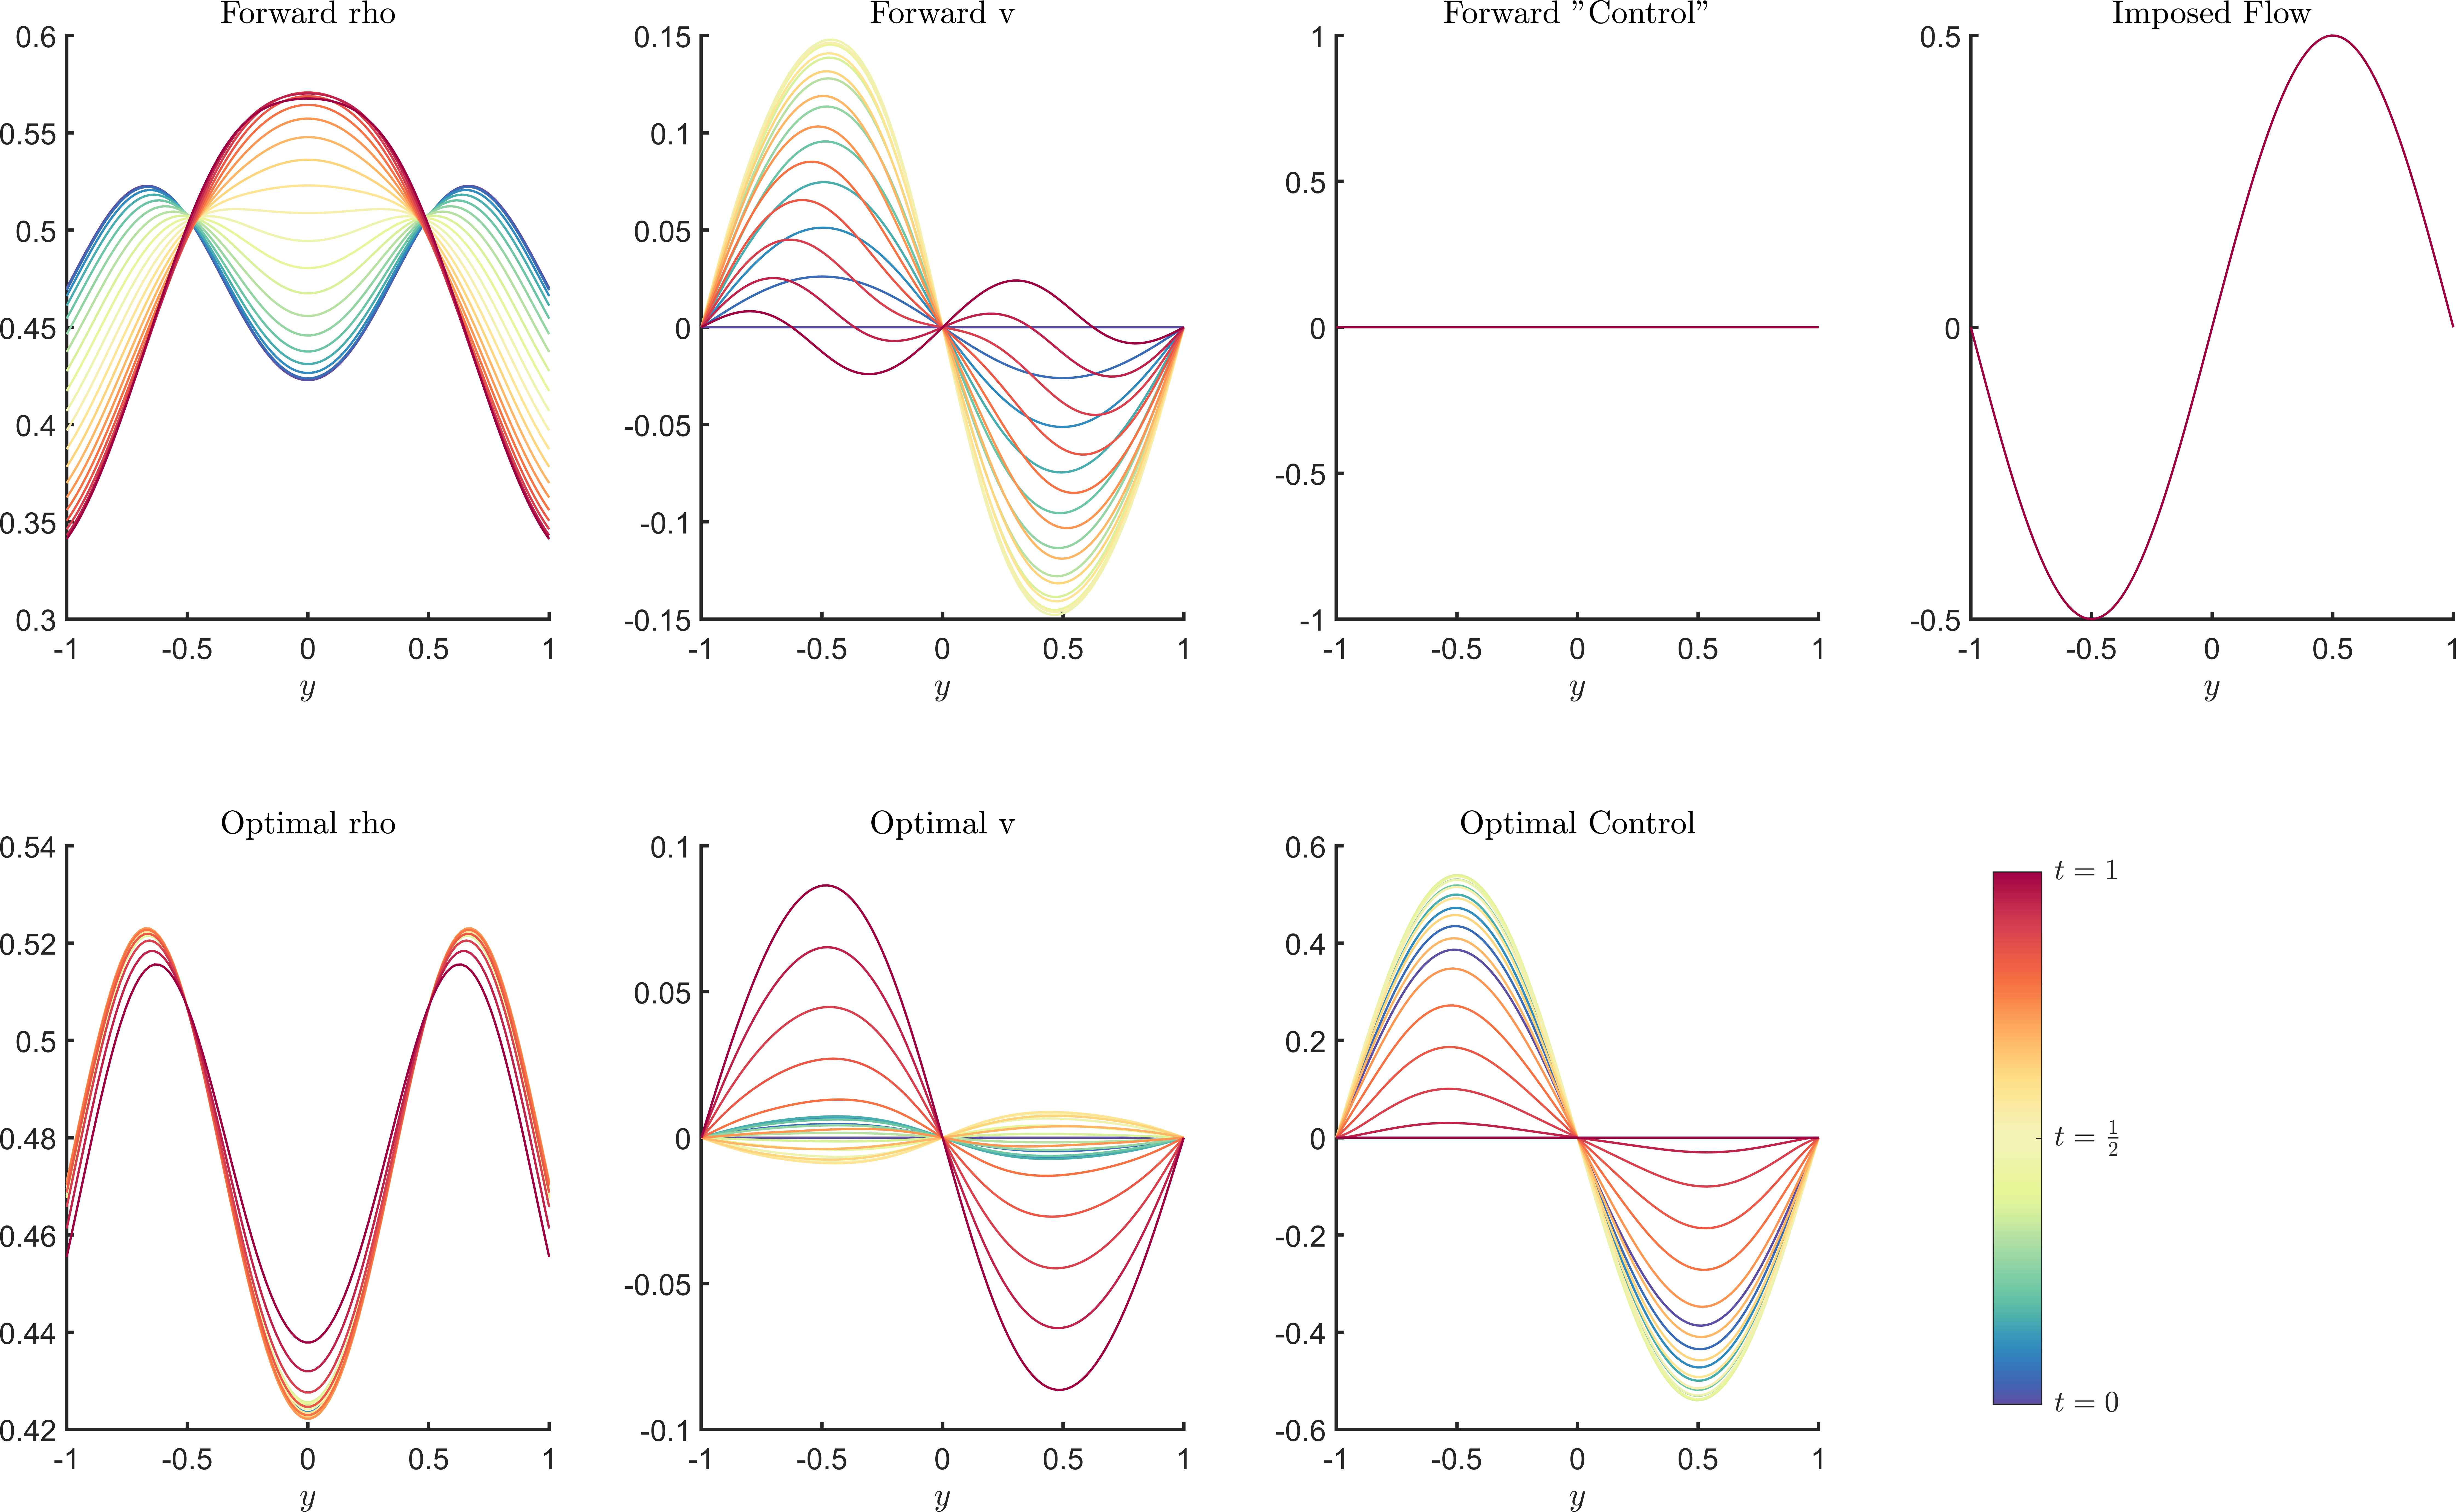
\includegraphics[scale=0.05]{Example3a.png}
	\caption{Example 3a ($\gamma = 0.1$, $\eta = 0.01$)}
	\label{fig3a}
\end{figure} 

\subsection{Fourth Test Problem}
Choosing $\Con$ to not satisfy the boundary conditions.
\begin{align*}
&\Sta_0 = \hat \Sta = \frac{1}{2.0507}e^{-0.5 \frac{2}{3 \pi}\sin((3/2)\pi y)}, \ \ V^{ext} =0.5 \frac{2}{3 \pi}\sin((3/2)\pi y)\\
&\Stav = \mathbf{0}, \ \  \mathbf{w} = \mathbf{0}\\
&\Con = 0.5
\end{align*}
For $\gamma = 0.1$, $\eta = 0.01$, this works, but Figure \ref{fig4} shows the issue with this. The gradient of the optimal control is steep, since it has to satisfy the boundary conditions. $J_FW = 0.0049$, $J_{Opt} = 1.7718 \times 10^{-4}$.

\begin{figure}
	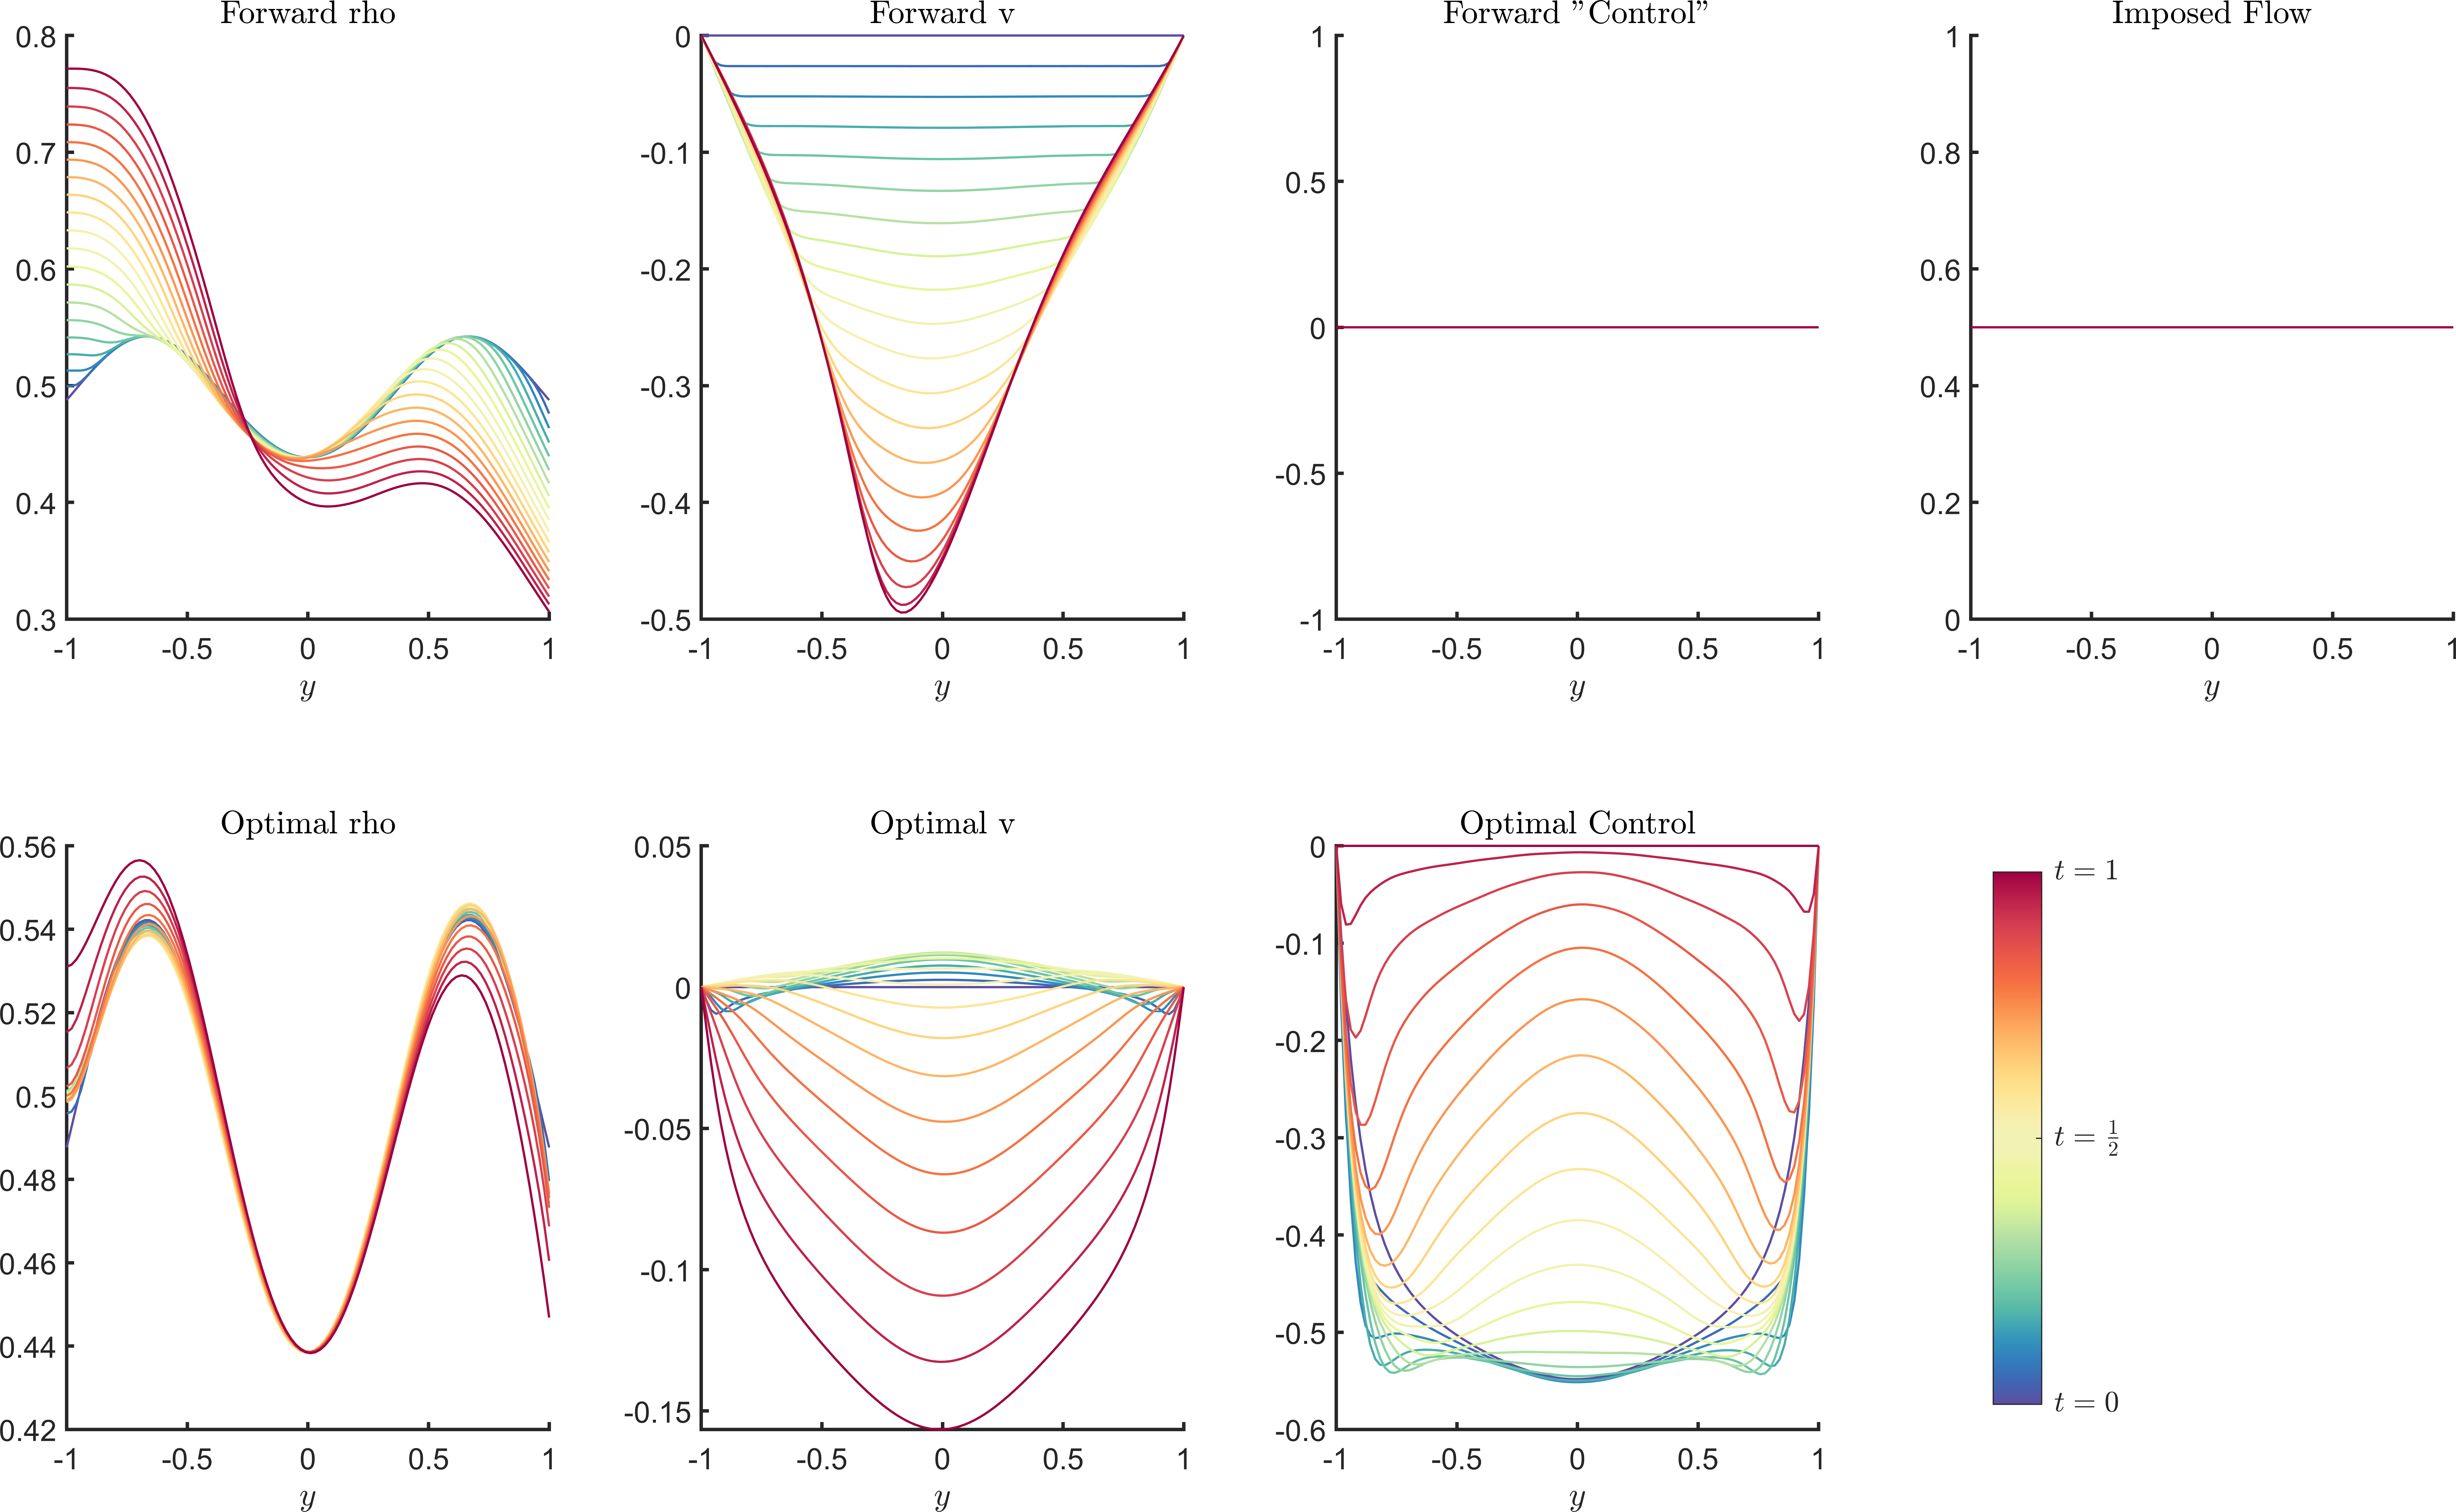
\includegraphics[scale=0.05]{Example4.png}
	\caption{Example 4 ($\gamma = 0.1$, $\eta = 0.01$)}
	\label{fig4}
\end{figure} 

\subsection{Fifth Test Problem}
Choosing a different potential than trig functions.
\begin{align*}
&\Sta_0 = \hat \Sta =  \frac{1}{4.0602}e^{- y^2 + 1}, \ \ V^{ext} = y^2 - 1\\
&\Stav = \mathbf{0}, \ \  \mathbf{w} = \mathbf{0}\\
&\Con = 0.5 \sin(\pi y) 
\end{align*}
This works as expected with $\gamma = 0.1$, $\eta = 0.01$ and we get $J_{FW} =0.0041$, $J_{Opt} = 9.9384 \times 10^{-5}$, see Figure \ref{fig5}.
\begin{figure}
	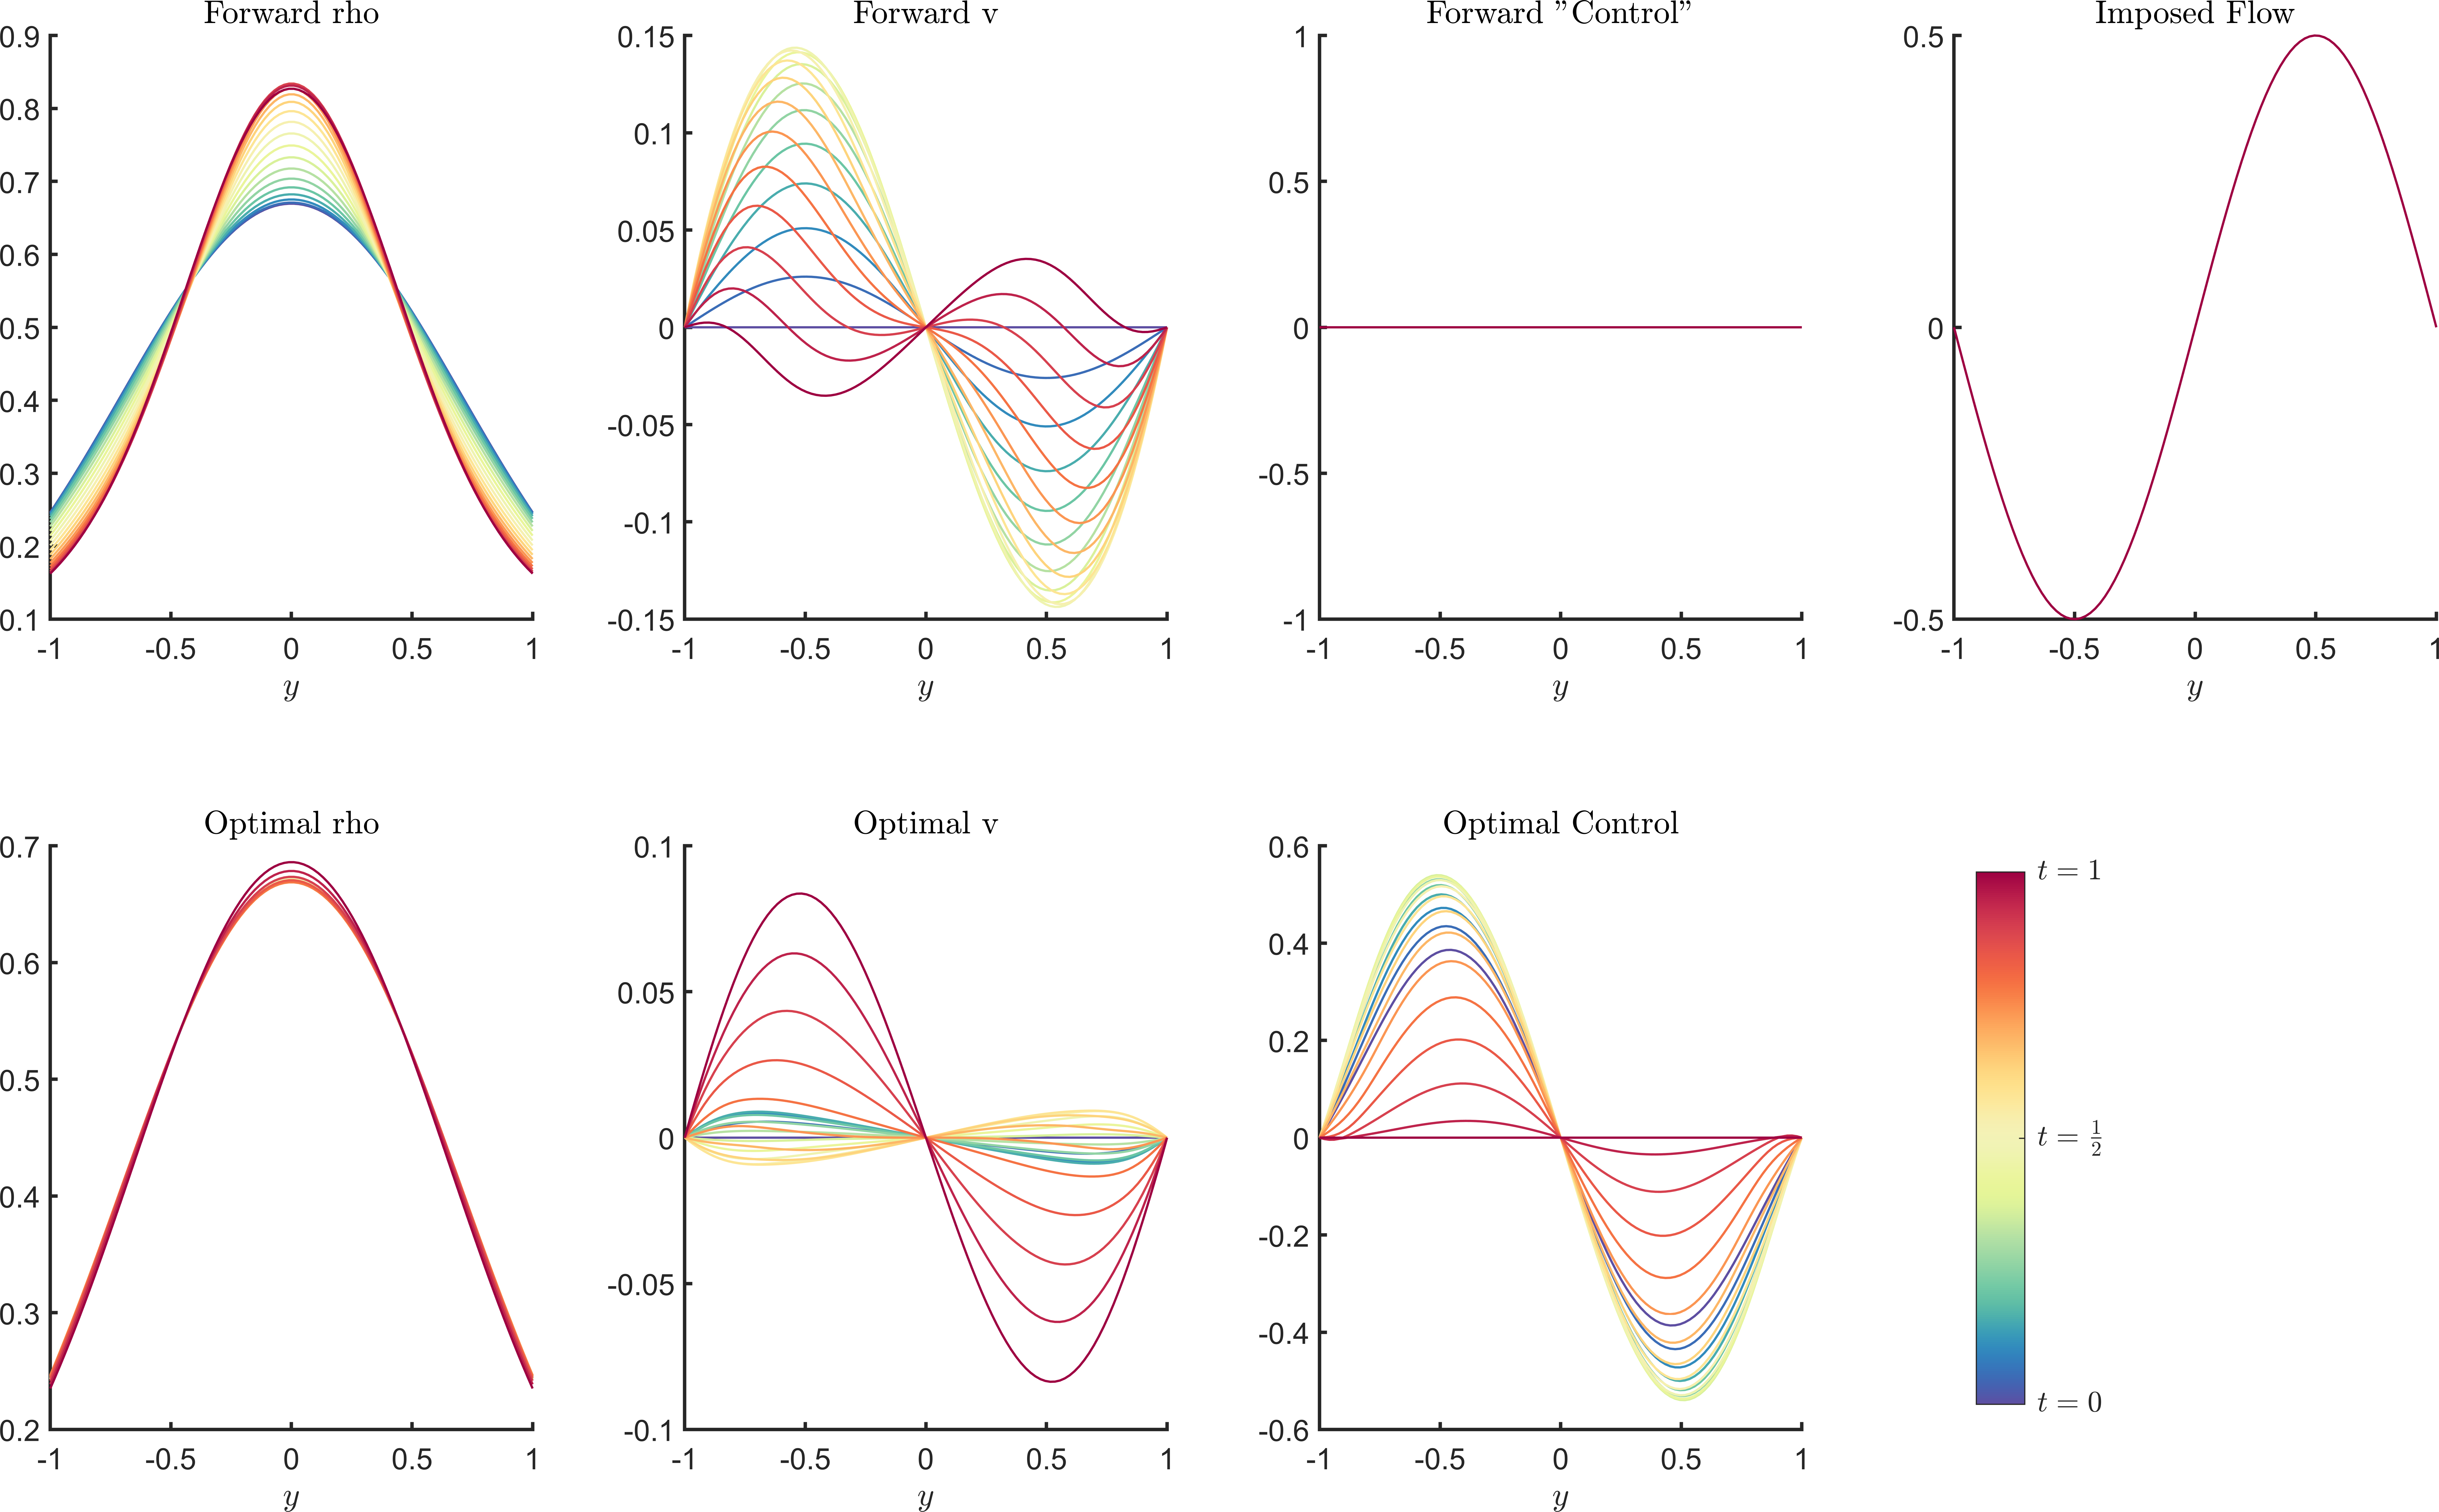
\includegraphics[scale=0.05]{Example5.png}
	\caption{Example 5 ($\gamma = 0.1$, $\eta = 0.01$)}
	\label{fig5}
\end{figure} 

\section{Interacting Problems}
\subsection{The Optimality System}
Here we have $\rho = e^s$. 
The forward equations are:
\begin{align*}
& \frac{\partial \Stav}{\partial t}= -  (\Stav \cdot \nabla)\Stav - \frac{1}{m} \nabla V_{ext} -\frac{1}{m}\Con -\frac{1}{m} \mathbf{w} - \frac{1}{m} \nabla s - \gamma \Stav +  \frac{\eta}{m} \nabla^2 \Stav \\
& - \frac{1}{m}\int_\Omega e^{s(r')} \nabla V_2(|r - r'|)dr'\\
&\frac{\partial s}{\partial t} = - \Stav \cdot \nabla s - \nabla \cdot \Stav  
\end{align*}
The first adjoint equation (in time $\tau$) is:
\begin{align*}
& \frac{\partial \Adjb}{\partial \tau} = - (e^s - \hat \rho)  + \nabla s \cdot \Adja + \nabla\cdot \Adja  +  \nabla \Adjb \cdot \Stav   - \int_\Omega e^{s(r')} (\Adja(r) - \Adja(r'))\cdot\nabla V_2(|r - r'|)dr'
\end{align*}
The second adjoint equation (in time $\tau$) is:
\begin{align*}
\frac{\partial \Adja}{\partial \tau} =& 
\frac{2 \eta}{m} \nabla \Adja \cdot \nabla s + \frac{\eta}{m} \Adja \cdot (\nabla s)^2 + \frac{\eta}{m} \Adja \cdot \nabla^2 s + \frac{\eta}{m} \nabla^2 \Adja \\
&  -\gamma  \Adja + \frac{1}{m} \nabla \Adjb - (\nabla \Stav)^\top\Adja + (\Stav \cdot \nabla)\Adja
\end{align*}
The gradient equation is:
\begin{align*}
\mathbf{w} = - \frac{1}{\beta} \Sta \Adja \quad \text{in} \quad \Sigma \quad \text{and on } \quad \partial\Sigma.
\end{align*}
Note that this is still in the original variable $\rho$. This is in line with the code.

\subsection{Third Test Problem - Revisited}
The choice of input is:
\begin{align*}
&\Sta_0 = \hat \Sta = \frac{1}{2.0507}e^{-0.5 \frac{2}{3 \pi}\sin((3/2)\pi y)}, \ \ V^{ext} =0.5 \frac{2}{3 \pi}\sin((3/2)\pi y)\\
&\Stav = \mathbf{0}, \ \  \mathbf{w} = \mathbf{0}\\
&\Con = 0.5 \sin(\pi y) 
\end{align*}
For $\gamma = 0.1$, $\eta = 0.01$, the configuration with $\kappa = 0$, without interactions, corresponds to Figure \ref{fig3a}.

Then, with $\kappa = 1$, we get $J_{FW} = 3.4647 \times 10^{-4}$, $J_{Opt} = 4.1156 \times 10^{-5}$, see Figure \ref{fig3I1a}.
Then, with $\kappa = -1$, we get $J_{FW} = 0.0149$, $J_{Opt} = 2.0372 \times 10^{-4}$, see Figure \ref{fig3In1a}.
It seems like repulsive particles are benefiting the target in this example, while attractive particles make it harder to reach.

\begin{figure}
	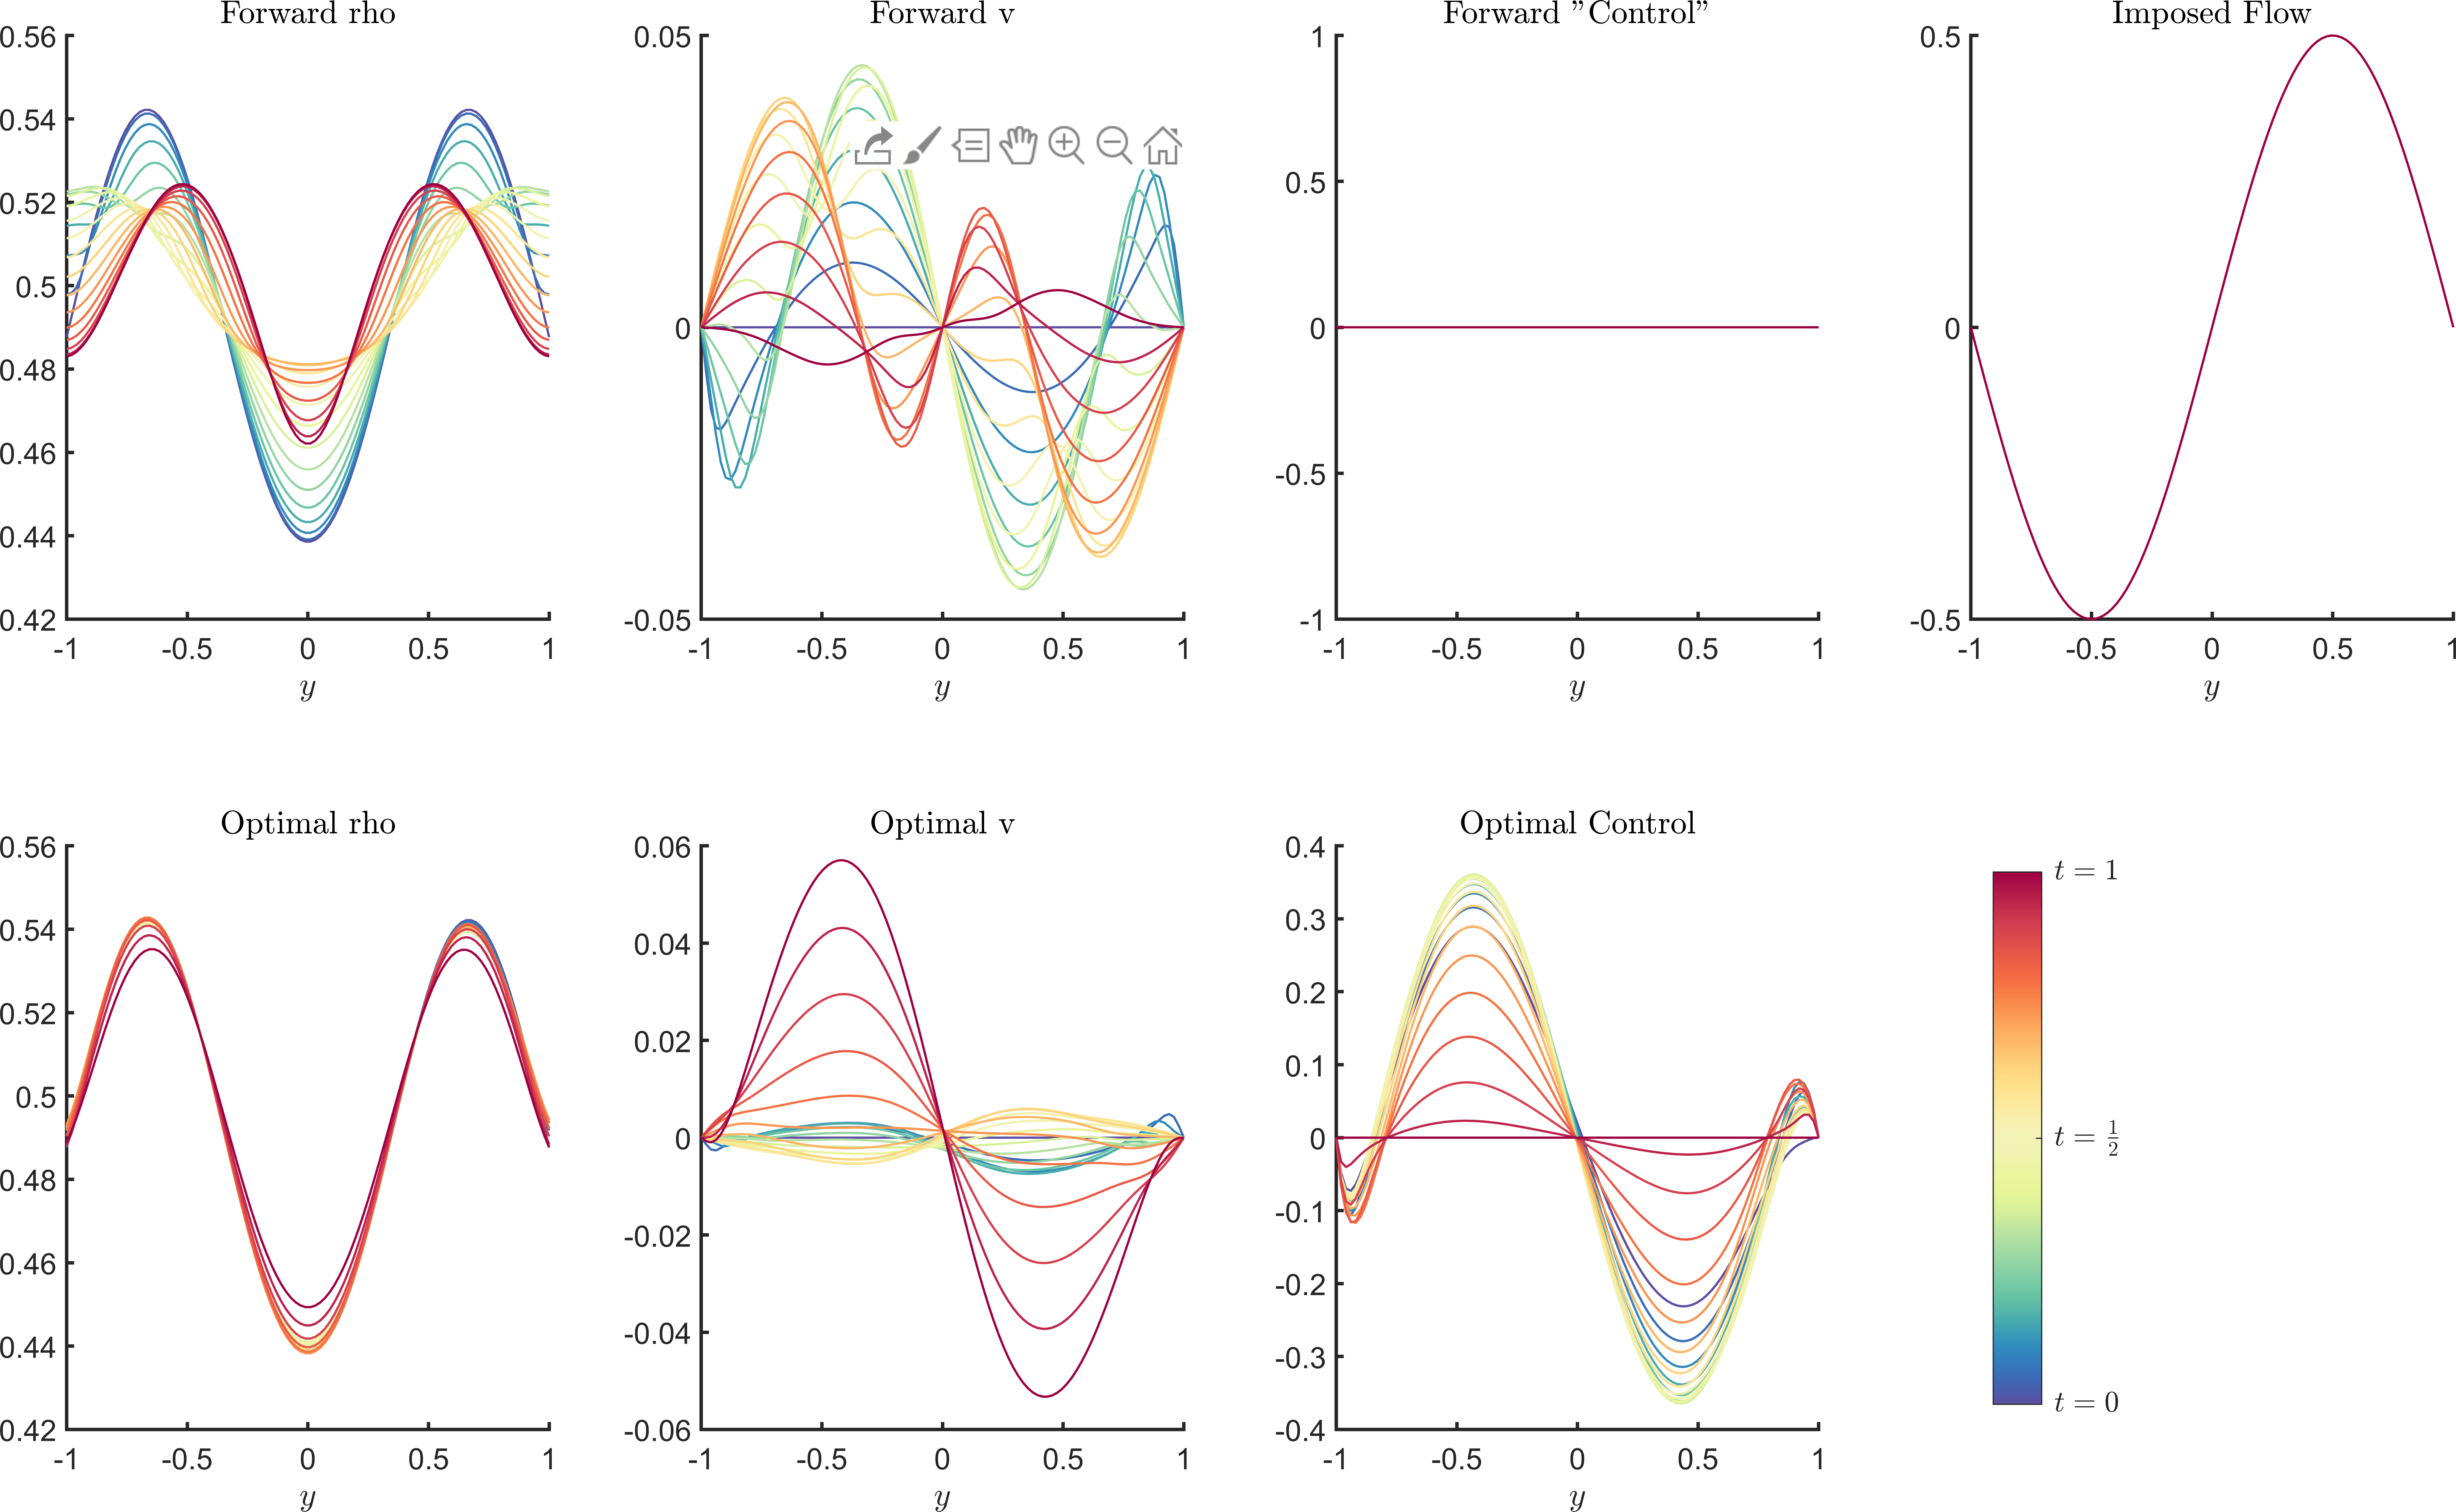
\includegraphics[scale=0.05]{ExampleI13.png}
	\caption{Example 3 with $\kappa = 1$ ($\gamma = 0.1$, $\eta = 0.01$)}
	\label{fig3I1a}
\end{figure} 
\begin{figure}
	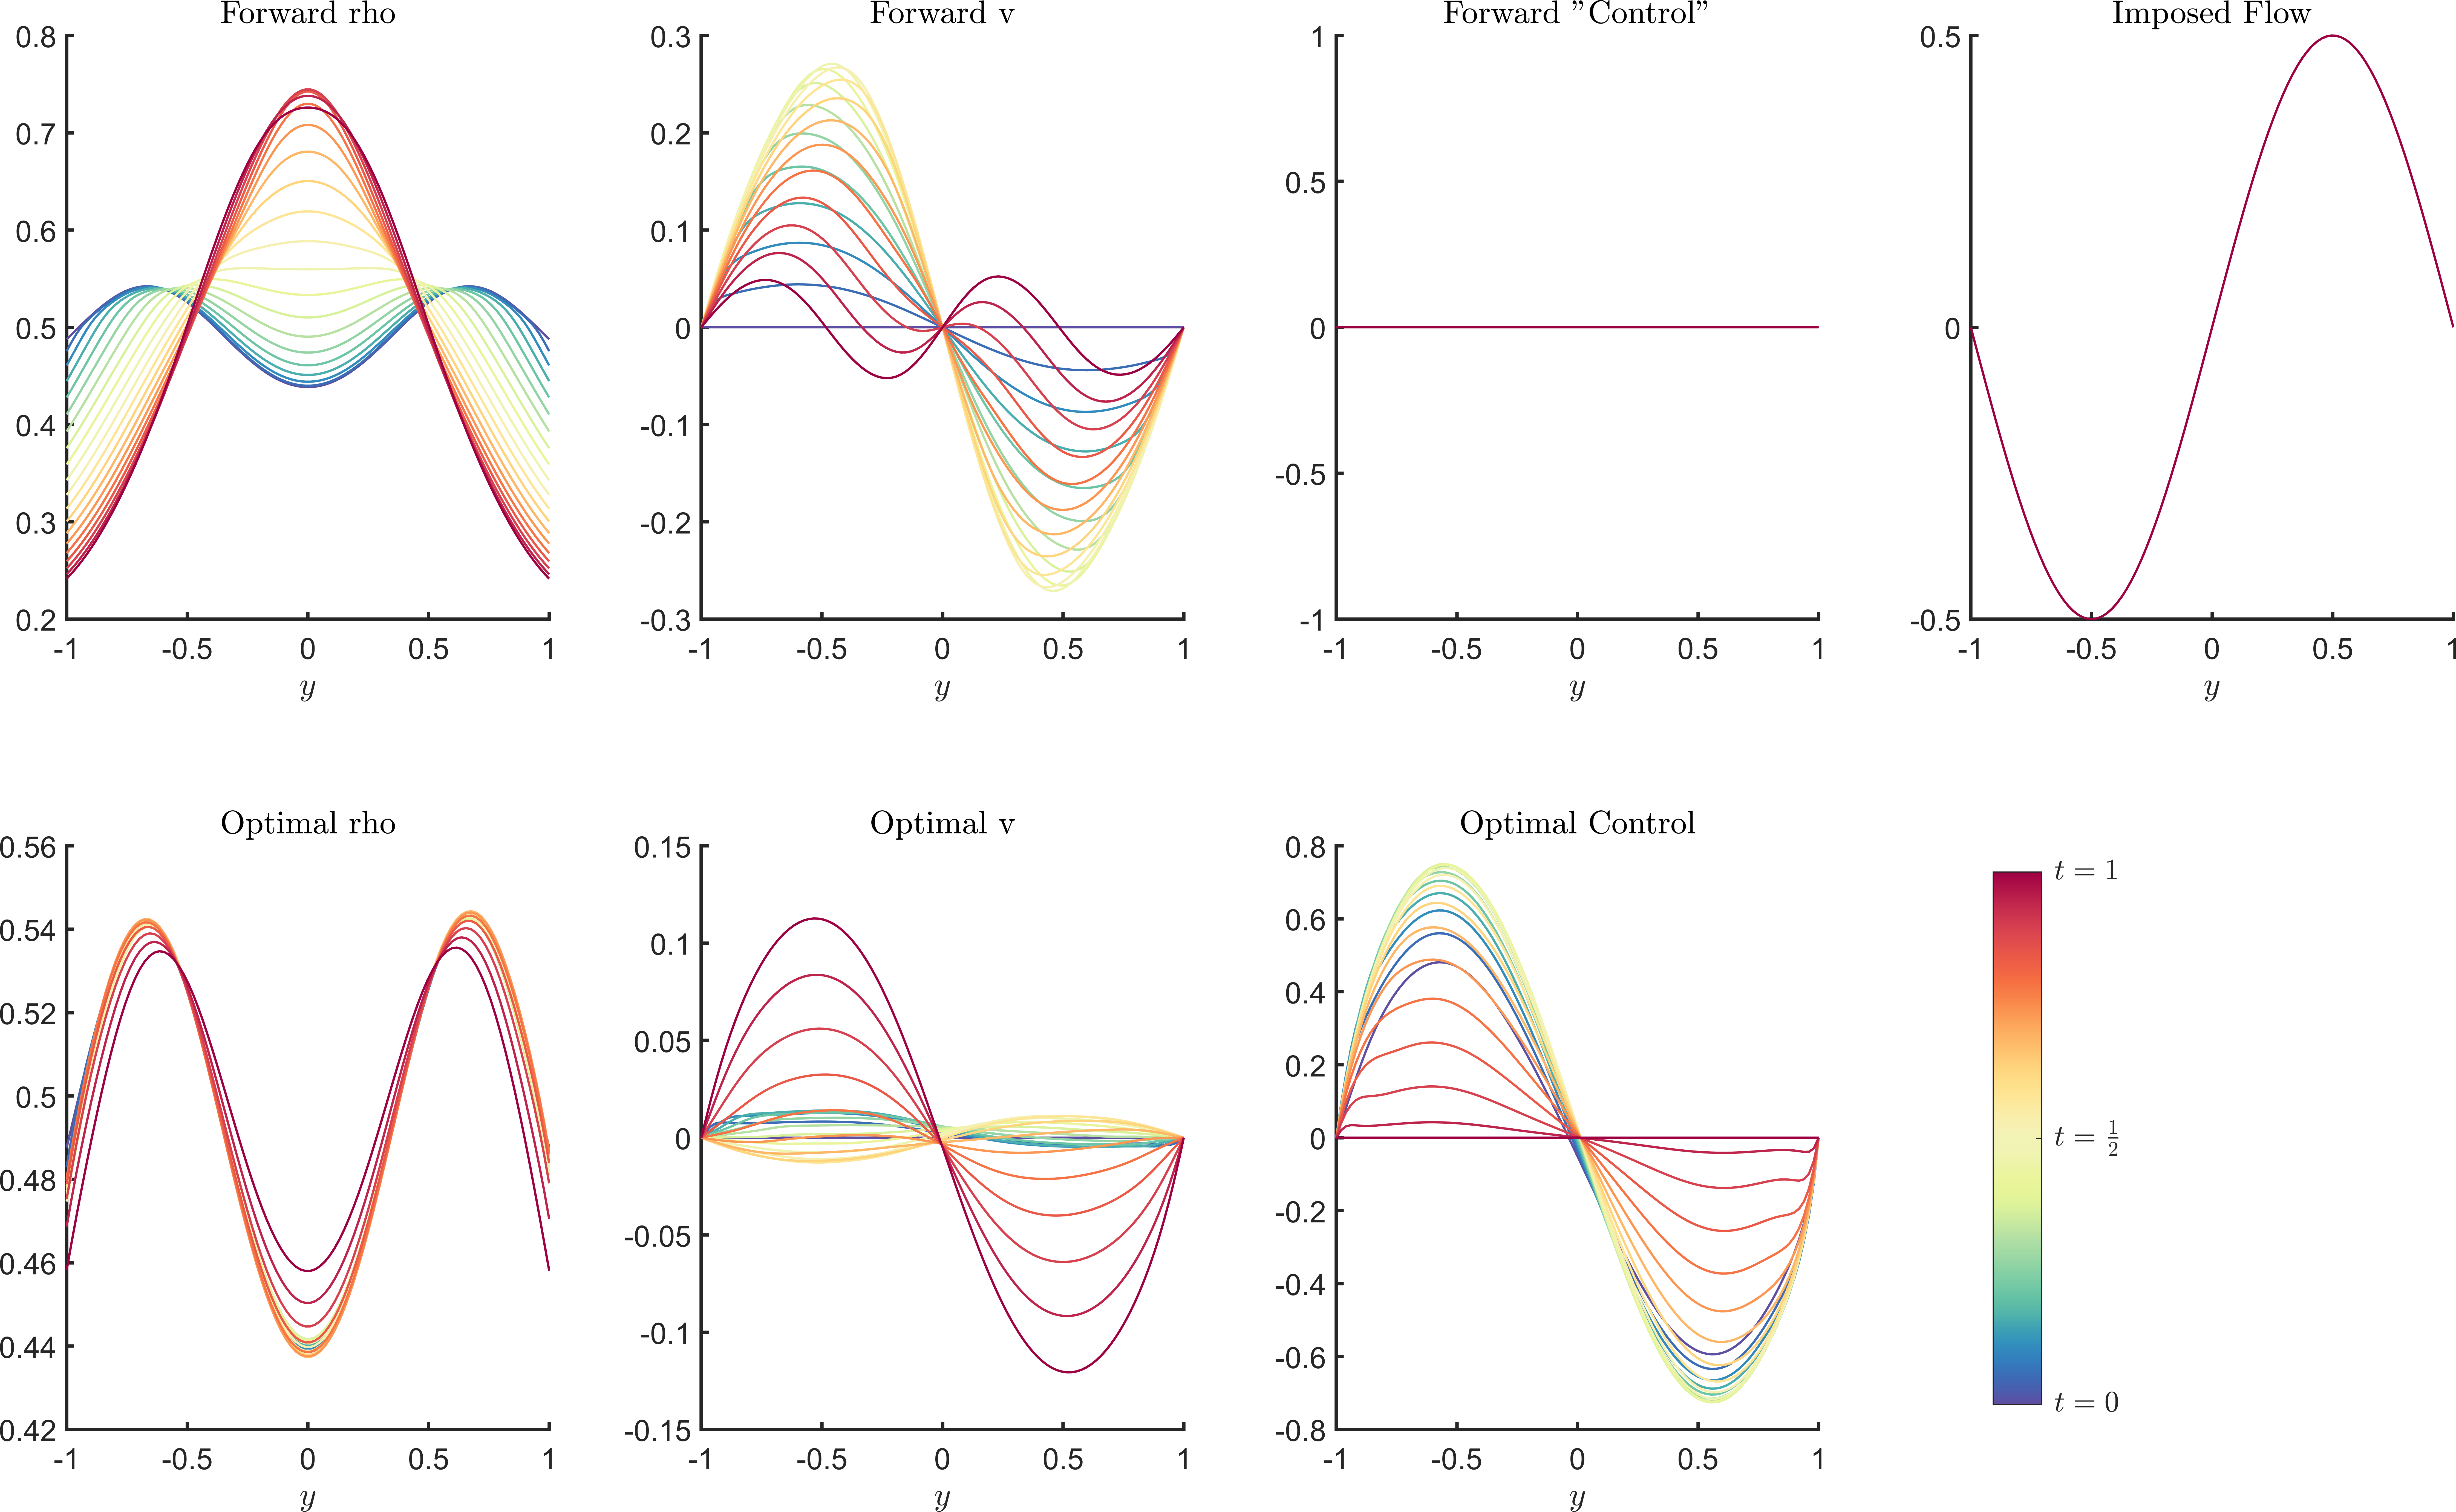
\includegraphics[scale=0.05]{ExampleIn13.png}
	\caption{Example 3 with $\kappa = -1$ ($\gamma = 0.1$, $\eta = 0.01$)}
	\label{fig3In1a}
\end{figure} 

\subsection{Fifth Test Problem - Revisited}
The choice of input is:
\begin{align*}
&\Sta_0 = \hat \Sta =  \frac{1}{4.0602}e^{- y^2 + 1}, \ \ V^{ext} = y^2 - 1\\
&\Stav = \mathbf{0}, \ \  \mathbf{w} = \mathbf{0}\\
&\Con = 0.5 \sin(\pi y) 
\end{align*}


For $\gamma = 0.1$, $\eta = 0.01$, the configuration with $\kappa = 0$, without interactions, corresponds to Figure \ref{fig5}.

Then, with $\kappa = 1$, we get $J_{FW} = 1.3521 \times 10^{-4}$, $J_{Opt} = 2.8400\times 10^{-5}$, see Figure \ref{fig5I1a}.
Then, with $\kappa = -1$, we get $J_{FW} = 0.0164$, $J_{Opt} = 2.2032 \times 10^{-4}$, see Figure \ref{fig5In1a}.
It seems like repulsive particles are benefiting the target also in this example, while attractive particles make it harder to reach.

\begin{figure}
	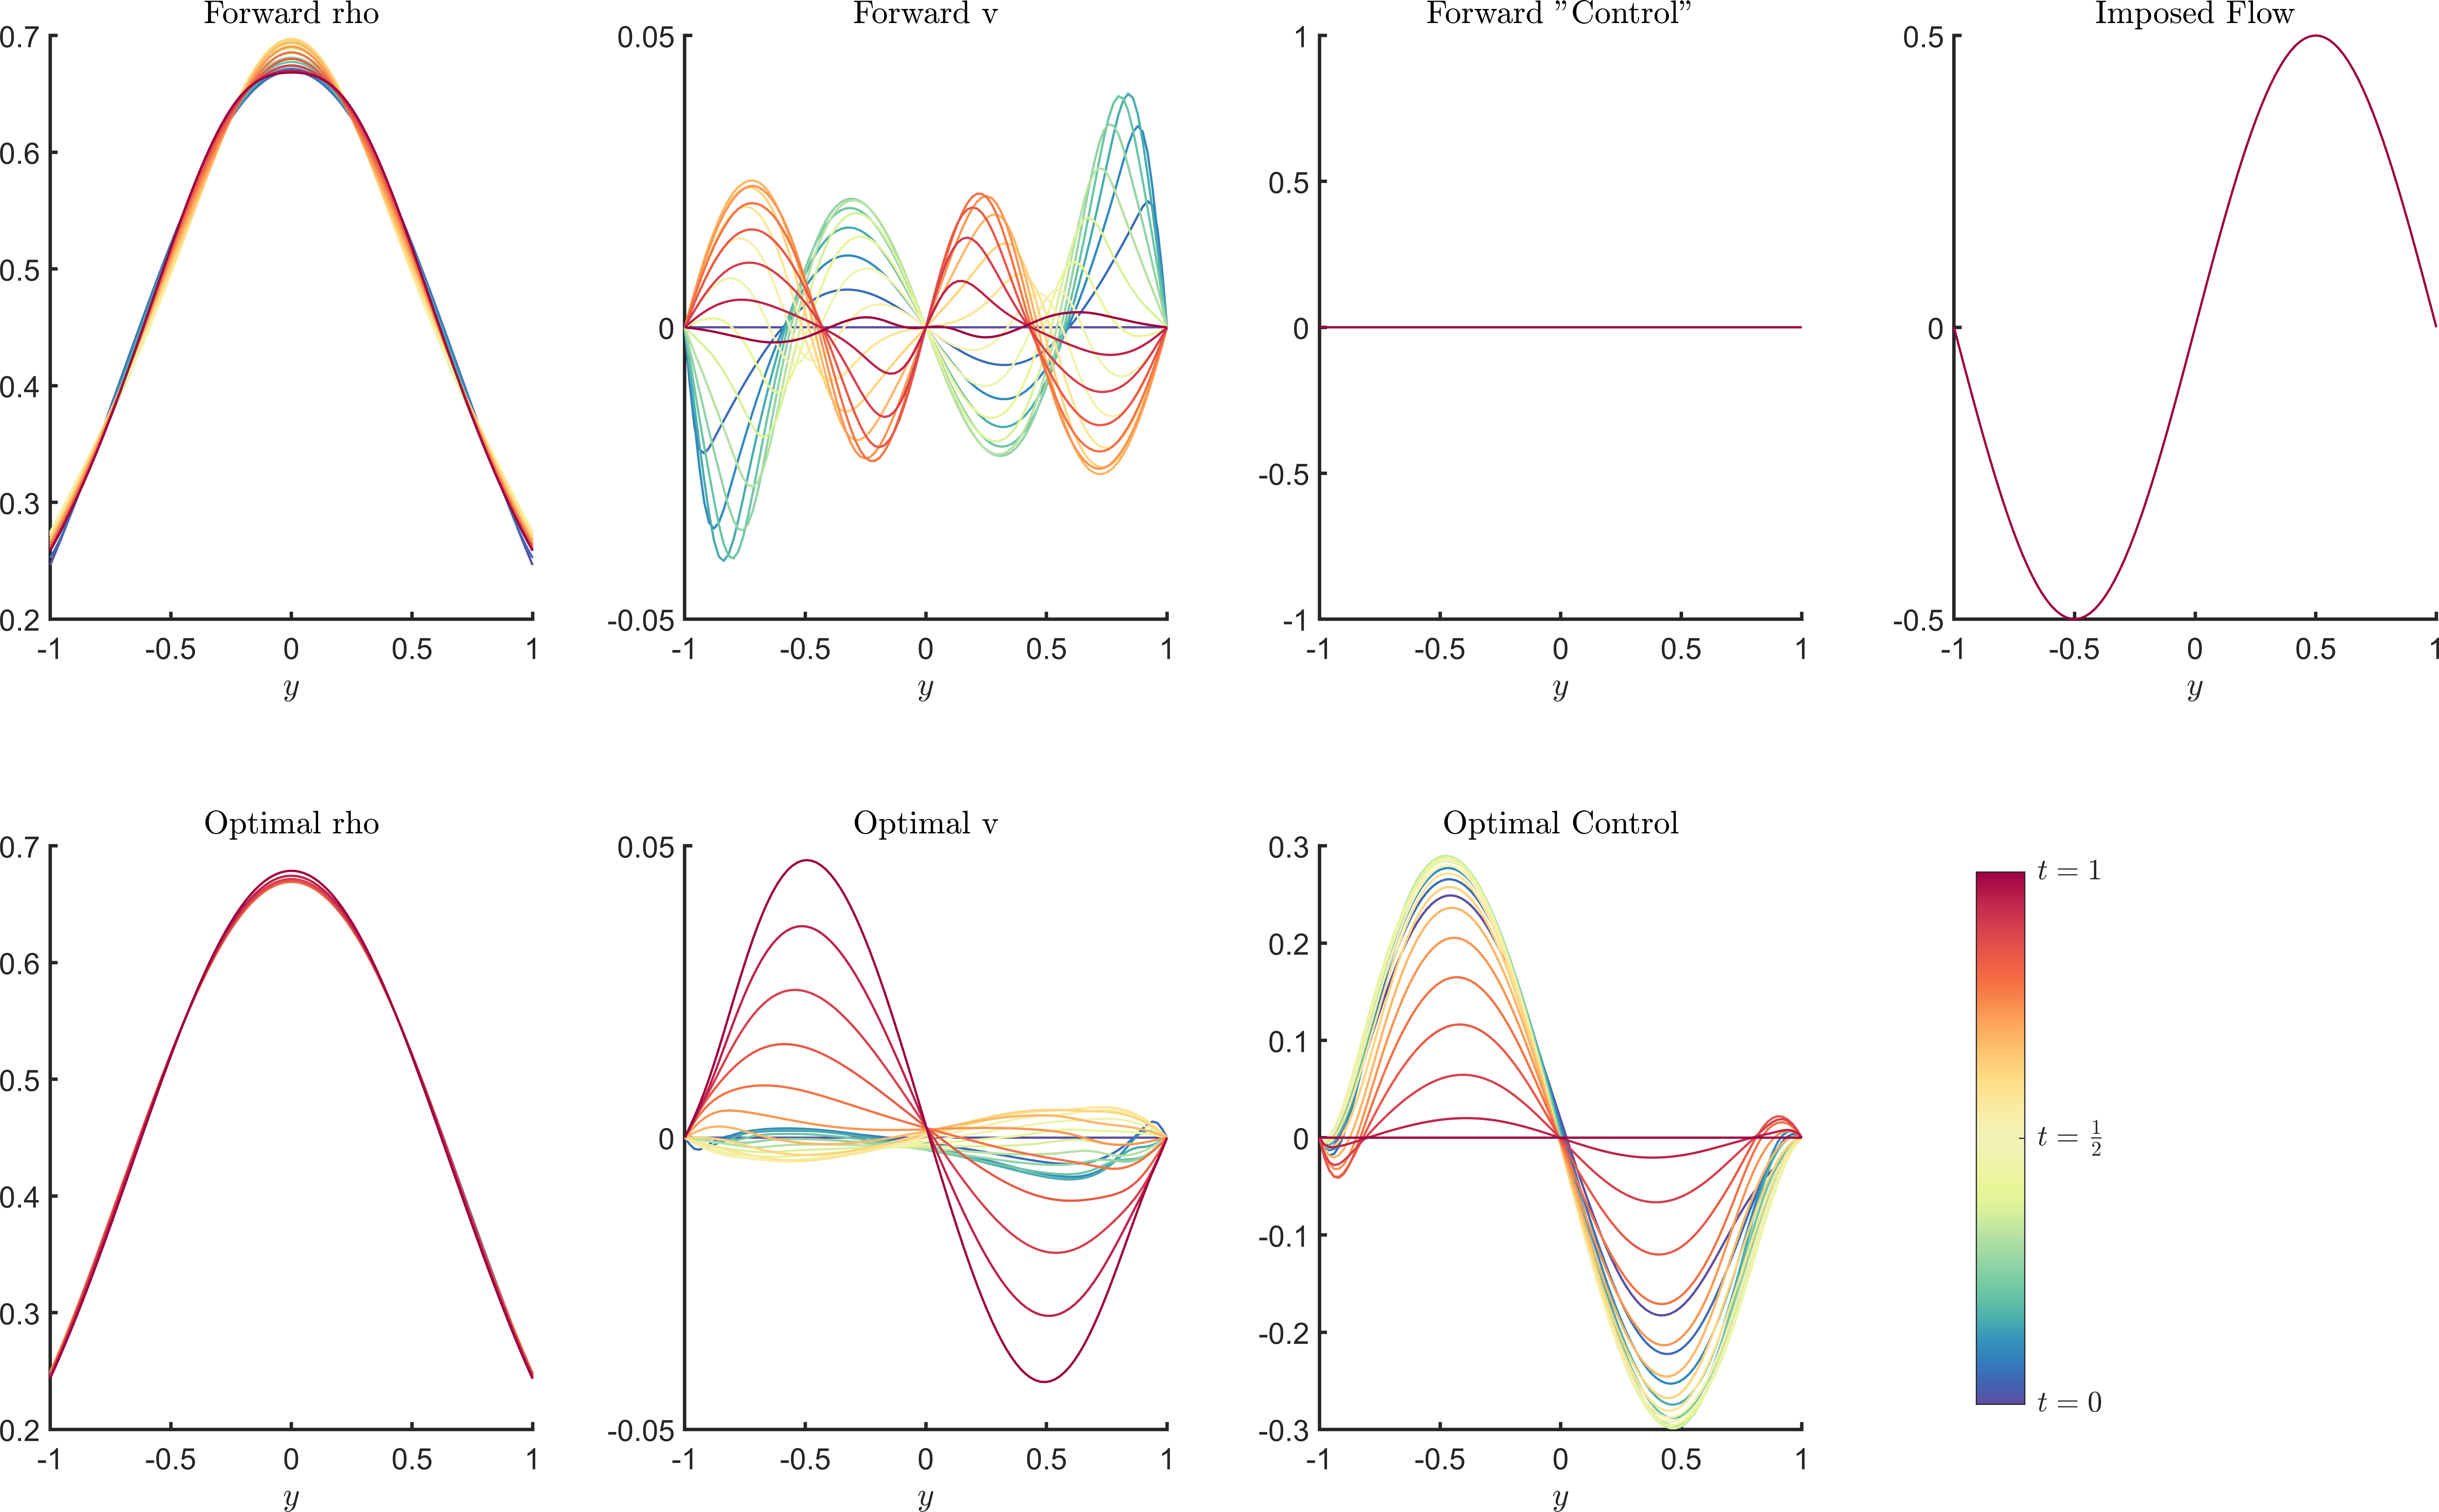
\includegraphics[scale=0.05]{ExampleI15.png}
	\caption{Example 5 with $\kappa = 1$ ($\gamma = 0.1$, $\eta = 0.01$)}
	\label{fig5I1a}
\end{figure} 
\begin{figure}
	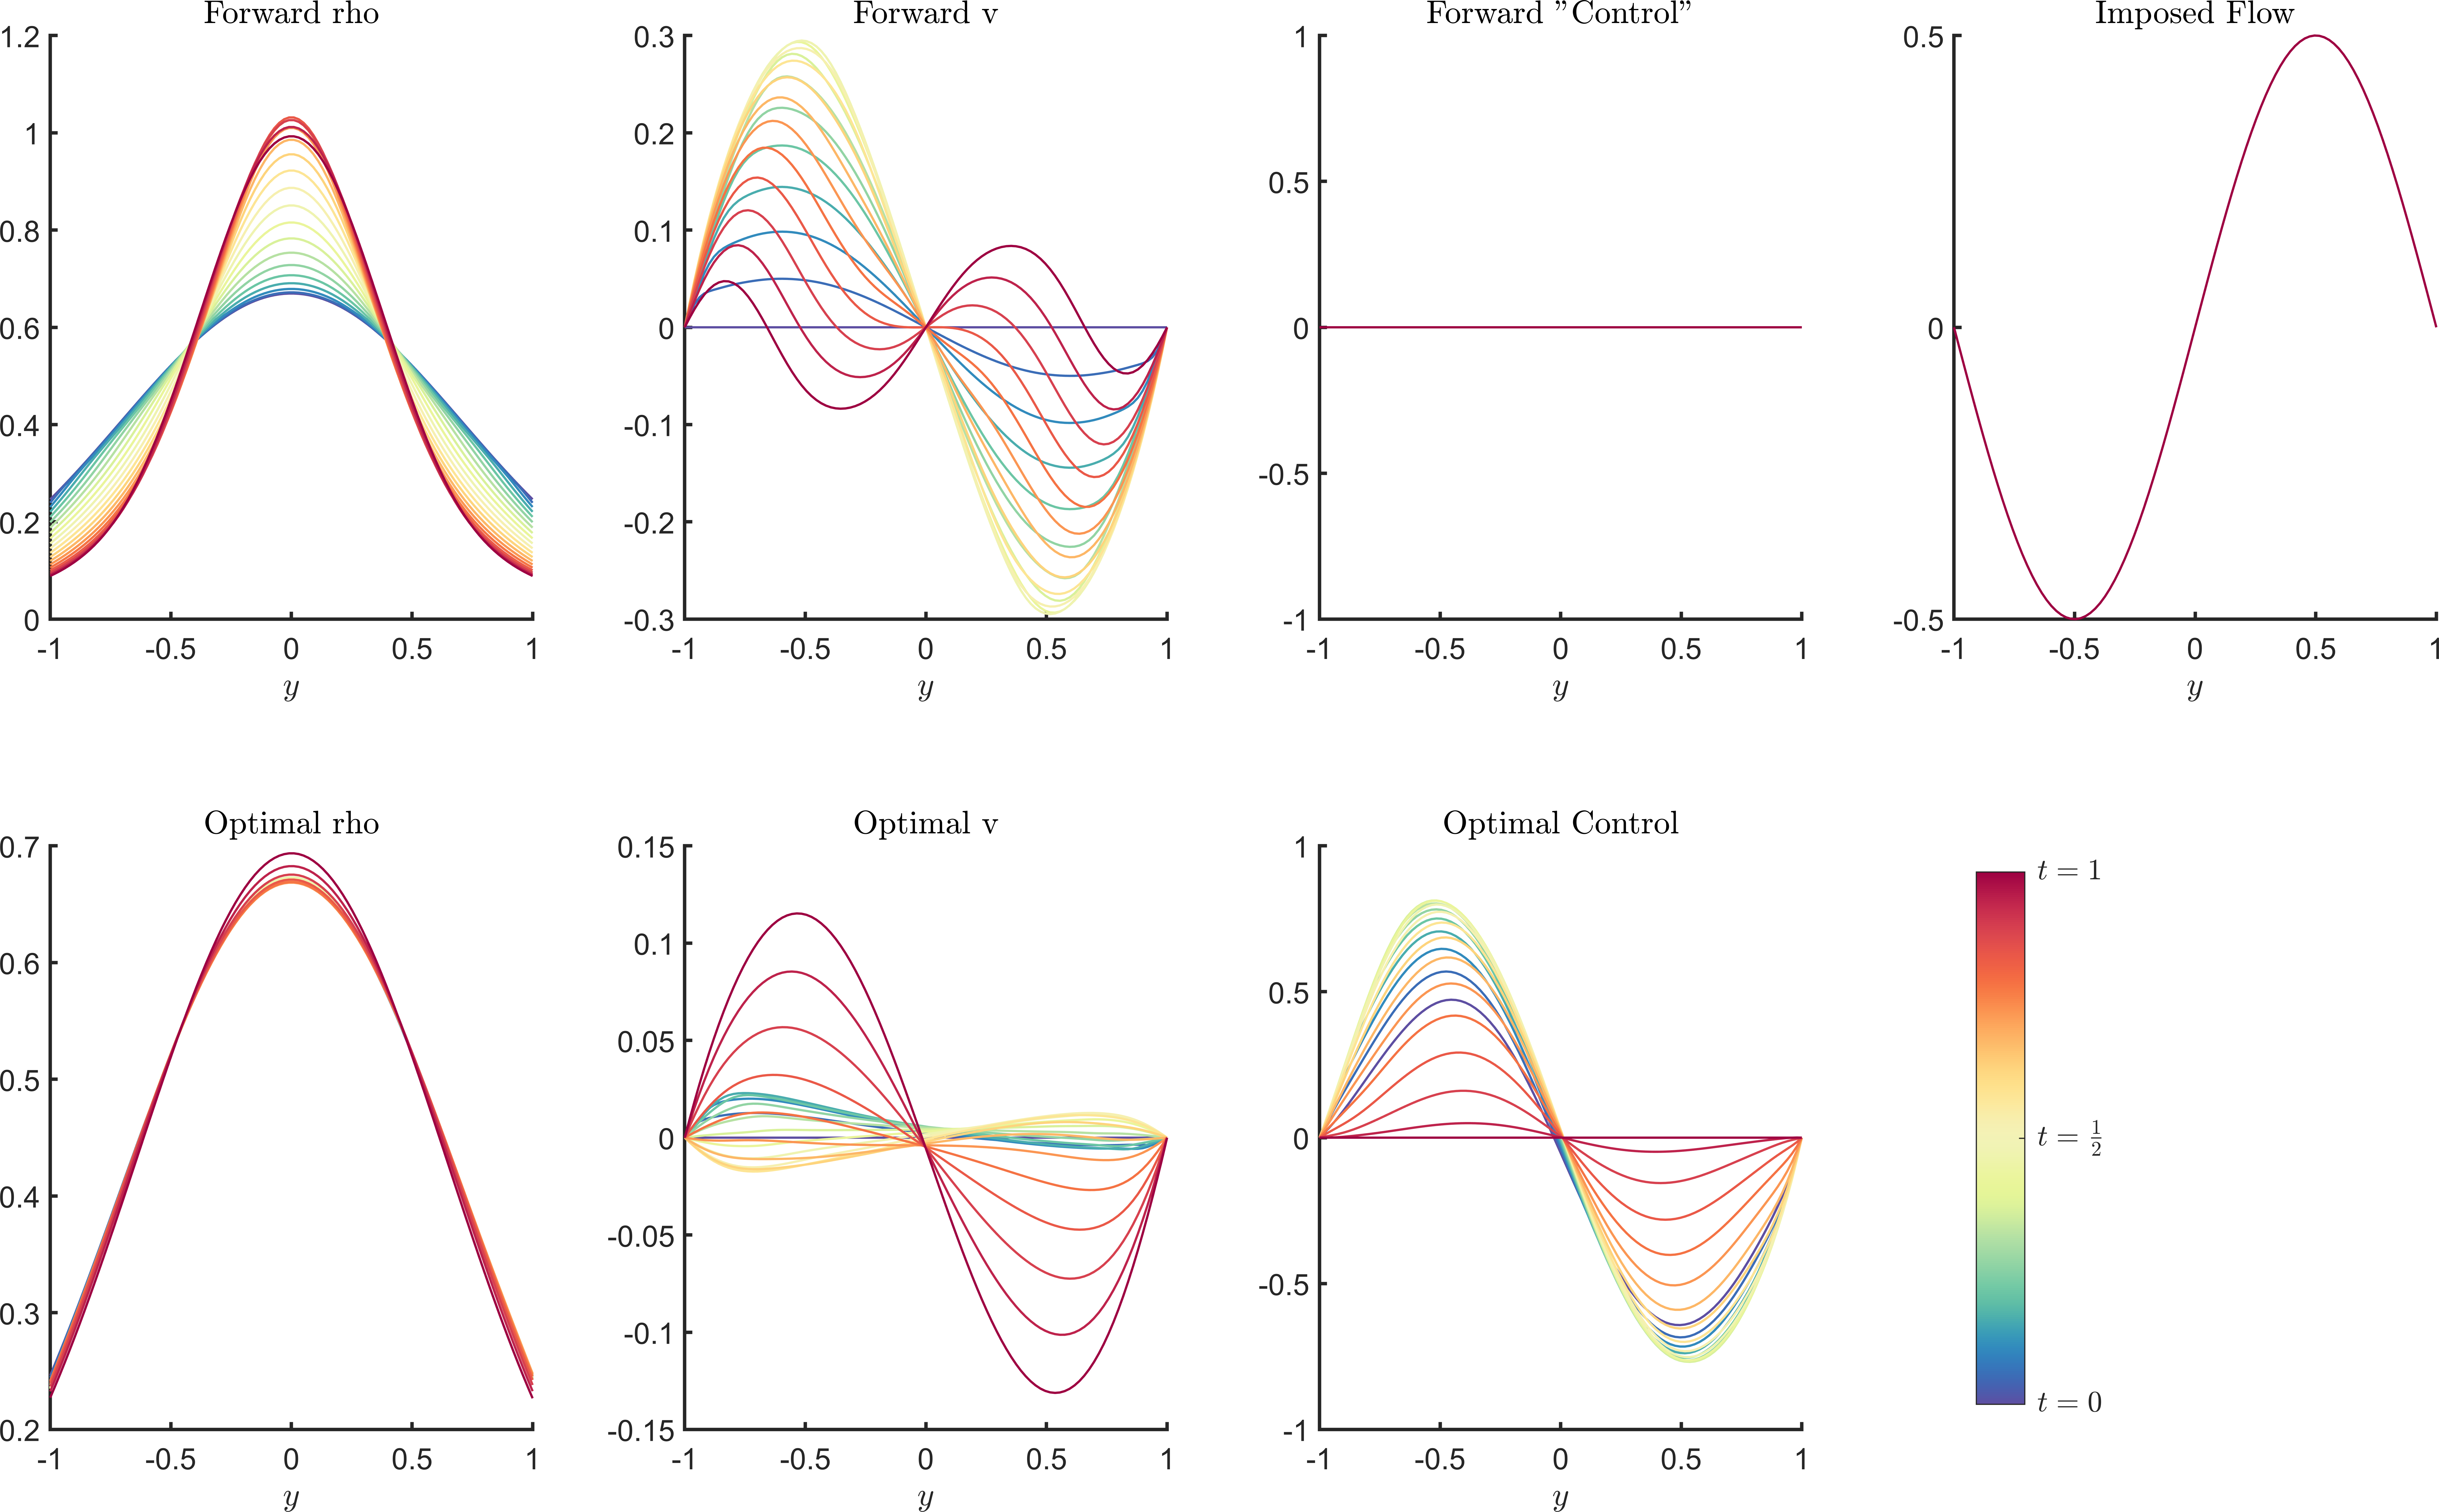
\includegraphics[scale=0.05]{ExampleIn15.png}
	\caption{Example 5 with $\kappa = -1$ ($\gamma = 0.1$, $\eta = 0.01$)}
	\label{fig5In1a}
\end{figure} 









\end{document}